\documentclass[11pt]{article}

\usepackage[margin=1in]{geometry}
\usepackage[T1]{fontenc}
\usepackage[utf8]{inputenc}
\usepackage{amsmath,amssymb}
\usepackage{booktabs}
\usepackage{array}
\usepackage{graphicx}
\usepackage{subcaption}
\usepackage{float}
\usepackage[section]{placeins}
\usepackage{hyperref}

\hypersetup{
    colorlinks=true,
    linkcolor=blue,
    citecolor=blue,
    urlcolor=blue
}

\title{\textbf{Adaptive Preconditioned Dynamics, Solution Geometry, and Generalization in Neural Networks}\\
\Large A Matched-Seed Study of SGD and Adam Across Parameter, Basin, Function, and Representation Geometry}
\author{Changyuan Yu(cy2812)~~~~~Xiangyu Liao(xl3581)\\Zhiliang Wang(zw3162)~~~~~Kevin Sun(ys3978)}
\date{May 2026}

\begin{document}
\maketitle

\begin{abstract}
Adaptive optimizers are often viewed as tools for faster convergence, but in over-parameterized neural networks they may also change which low-loss solution is selected. We study this question by comparing SGD with momentum and Adam as two preconditioned stochastic dynamics under a matched-seed protocol on Fashion-MNIST. Mathematically, SGD applies scalar spatial preconditioning while Adam applies a time-varying diagonal preconditioner, and a local quadratic analysis shows that this changes the effective error dynamics through $e_{t+1}\approx (I-P_tH)e_t$. Empirically, Adam moves farther from initialization, traverses a longer path, and selects more dispersed parameter regions. We then test whether these differences persist under a loss-matched control, correspond to Hessian and perturbation-based flatness, imply basin separation through linear mode connectivity, and survive at the function and representation levels through prediction disagreement, symmetric KL, logit cosine, feature-kernel alignment, and centered linear CKA. The results show that optimizer-induced parameter geometry can be substantial in the MLP and weaker in the SmallCNN, but it does not by itself determine generalization. Generalization is mediated by loss level, architecture, basin connectivity, learned functions, and learned representations.
\end{abstract}

\section{Introduction}

Modern neural networks are typically over-parameterized: they can fit the training data in many different ways, often with many parameter settings achieving nearly zero training error. In this regime, the optimizer does more than minimize the empirical risk. It also helps select which interpolating or near-interpolating solution the training procedure reaches. This selection effect is commonly called the \emph{implicit bias} or \emph{implicit regularization} of the optimization algorithm.

Here we ask whether adaptive optimizers change that implicit bias. We focus on the comparison between SGD with momentum and Adam. SGD applies one global learning-rate scale to all coordinates of the stochastic gradient. Adam instead rescales each coordinate using estimates of the first and second moments of recent gradients \cite{kingma2015adam}. This coordinate-wise adaptation is often helpful in early optimization, especially when gradients vary strongly across layers or coordinates. At the same time, it may also change the geometry of the final solution and therefore affect generalization.

The overall project question is:
\begin{quote}
\emph{Do adaptive optimizers alter the implicit bias and generalization of neural networks?}
\end{quote}
We divide this broad question into three parts that frame the original study:
\begin{enumerate}
    \item \textbf{Early-stage convergence.} Does Adam converge faster than SGD at the beginning of training?
    \item \textbf{Solution geometry.} If Adam is faster, does it reach a different kind of solution, or only the same solution earlier?
    \item \textbf{Generalization.} Do the observed geometric differences explain differences in test performance or train--test gap?
\end{enumerate}
The extended report (Parts~IV--IX) deepens this question by following the optimizer-induced effect through additional layers of evidence: trajectory geometry (path length, update norm), a loss-matched control that decouples geometry from training-loss level, perturbation flatness as an operational check on the Hessian-trace proxy, linear mode connectivity to test for basin separation, and function-space and representation-space comparisons that ask whether parameter differences propagate to the learned predictor and to internal feature geometry. The contributions are accordingly:
\begin{enumerate}
    \item We formulate SGD and Adam as two preconditioned stochastic dynamics and develop a local quadratic analysis $e_{t+1}\approx (I-P_tH)e_t$ that explains why a time-varying diagonal preconditioner can change the selected low-loss solution.
    \item We use matched seeds (shared initialization, shared minibatch order) to isolate optimizer-induced effects from initialization and batch-order randomness.
    \item We characterize parameter-space geometry through distance from initialization, cumulative path length, directness ratio, Hessian curvature proxies, and inter-seed dispersion, and test fairness via a loss-matched control and an update-norm control.
    \item We probe operational geometry through perturbation flatness and linear mode connectivity, separating Hessian-based curvature claims from actual robustness and basin connectivity.
    \item We compare the final models in function and representation space using prediction disagreement, symmetric KL, logit cosine similarity, feature-kernel alignment, and centered linear CKA, organizing the results in a three-level synthesis (parameter / basin / function--representation).
\end{enumerate}

The answer is not simply that Adam is better or worse than SGD. Instead, the experiments show a conditional pattern. In the MLP, Adam has a clear early optimization advantage and lands in much flatter solutions according to the Hessian proxies we measure ($5\times$ lower $\lambda_{\max}$, $6\times$ lower trace). Even so, these geometric differences do not produce a clear generalization advantage: test accuracy and train--test gap differ by less than the observed seed-to-seed variation, which is not fully explained by a naive flat-minima interpretation. In the CNN, Adam is still slightly faster in training loss, but its dominant Hessian eigenvalue is actually higher than SGD's, while both optimizers reach similar test accuracy and generalization gaps. In other words, adaptive optimization changes the training trajectory and the selected parameter region, but whether this geometric change matters for generalization depends on architecture.

\section{Background and Problem Description}

\subsection{SGD and Adam}

Let the training set be $\{(x_i,y_i)\}_{i=1}^n$, and let $f_\theta$ be the neural network with parameters $\theta$. The empirical risk minimized during training is
\[
\widehat L(\theta)
= \frac{1}{n}\sum_{i=1}^n \ell(f_\theta(x_i),y_i),
\]
where $\ell$ is the cross-entropy loss. Since full-batch gradients are expensive, both SGD and Adam use minibatches. For a minibatch $B_t$, the minibatch loss is
\[
\widehat L_{B_t}(\theta)
= \frac{1}{|B_t|}\sum_{i\in B_t}\ell(f_\theta(x_i),y_i),
\]
and its gradient is an unbiased estimate of the full training gradient under uniform sampling:
\[
\mathbb{E}_{B_t}\big[\nabla \widehat L_{B_t}(\theta)\big]
= \nabla \widehat L(\theta).
\]

Let $\theta_t$ denote the parameter vector at update step $t$, and let
\[
g_t = \nabla_\theta \widehat L_{B_t}(\theta_t)
\]
be the stochastic gradient on minibatch $B_t$. In its simplest form, SGD uses
\[
\theta_{t+1} = \theta_t - \eta g_t,
\]
where $\eta$ is a global learning rate. In our experiments we use SGD with momentum, so the practical update includes an exponentially smoothed velocity, but the important feature remains that the gradient coordinates share a common scale.

More explicitly, SGD with momentum can be written as
\begin{align}
u_t &= \mu u_{t-1} + g_t,\\
\theta_{t+1} &= \theta_t - \eta u_t,
\end{align}
where $\mu$ is the momentum coefficient. Even with momentum, the step is still scaled by the same scalar learning rate $\eta$ in every coordinate. In matrix notation, this corresponds to using a scalar preconditioner $\eta I$.

The velocity recursion also shows why momentum changes the effective scale of the update. Expanding the recursion gives
\[
u_t
= g_t+\mu g_{t-1}+\mu^2 g_{t-2}+\cdots+\mu^{t-1}g_1.
\]
Thus $u_t$ is an exponentially decayed accumulation of past stochastic gradients. If the gradient were constant, $g_t=g$, then
\[
u_t
= \frac{1-\mu^t}{1-\mu}g
\quad\Longrightarrow\quad
u_t\to \frac{1}{1-\mu}g.
\]
For $\mu=0.9$, the steady-state velocity scale is about $10$ times the raw gradient scale, which is why the learning rate and momentum coefficient must be interpreted together. The important point for our comparison is that this amplification is still global: every coordinate is multiplied by the same scalar $\eta$ after the velocity is formed.

Adam maintains exponential moving averages of the gradient and squared gradient:
\begin{align}
m_t &= \beta_1 m_{t-1} + (1-\beta_1)g_t,\\
v_t &= \beta_2 v_{t-1} + (1-\beta_2)g_t^{\odot 2}.
\end{align}
After bias correction, Adam updates by
\begin{align}
\hat m_t &= \frac{m_t}{1-\beta_1^t},\\
\hat v_t &= \frac{v_t}{1-\beta_2^t},
\end{align}
and
\[
\theta_{t+1}
= \theta_t - \alpha \frac{\hat m_t}{\sqrt{\hat v_t}+\varepsilon}.
\]
Equivalently, Adam applies a diagonal, time-varying preconditioner:
\[
\theta_{t+1}
= \theta_t - \alpha D_t \hat m_t,
\qquad
D_t = \operatorname{diag}\left(\frac{1}{\sqrt{\hat v_{t,i}}+\varepsilon}\right)_i.
\]
Thus Adam normalizes each coordinate by an estimate of its recent gradient magnitude. The effective learning rate in coordinate $i$ is approximately
\[
\eta_{t,i}^{\mathrm{Adam}}
= \frac{\alpha}{\sqrt{\hat v_{t,i}}+\varepsilon}.
\]
Coordinates with consistently large gradients are damped, while coordinates with small or sparse gradients can receive relatively larger effective steps. In practice, this helps explain why Adam often reduces training loss quickly. It also suggests that Adam may follow a different path through parameter space than SGD.

The bias-correction terms in Adam are also mathematically important. Because $m_0=v_0=0$, the raw moving averages are biased toward zero during the first iterations. For example, if the gradient were constant, $g_t=g$, then
\[
m_t
= (1-\beta_1)\sum_{k=0}^{t-1}\beta_1^k g
= (1-\beta_1^t)g.
\]
Dividing by $1-\beta_1^t$ therefore recovers $g$ in this idealized case. The same calculation applies to $v_t$ with $\beta_2$ and $g^{\odot 2}$. This is why Adam uses $\hat m_t$ and $\hat v_t$ rather than the raw moment estimates during the update.

\subsection{Preconditioned Dynamics View}

A useful mathematical way to compare the two optimizers is through preconditioned first-order dynamics. A general preconditioned stochastic update can be written as
\[
\theta_{t+1}
=
\theta_t - P_t q_t,
\]
where $q_t$ is a gradient-like direction and $P_t$ is a positive scaling operator applied before the parameter update. For SGD with momentum,
\[
q_t=u_t,\qquad P_t=\eta I.
\]
For Adam,
\[
q_t=\hat m_t,\qquad
P_t=\alpha D_t,
\qquad
D_t=\operatorname{diag}\left(\frac{1}{\sqrt{\hat v_{t,i}}+\varepsilon}\right)_i.
\]
Thus the central mathematical contrast is not only ``momentum versus moments,'' but scalar preconditioning versus diagonal, time-varying preconditioning.

This distinction matters even in a simple local quadratic model. Suppose that near a point $\theta^\star$ the empirical loss is approximately
\[
\widehat L(\theta)
\approx
\widehat L(\theta^\star)
+
\frac{1}{2}(\theta-\theta^\star)^\top H(\theta-\theta^\star),
\]
where $H\succeq 0$. Full-batch gradient descent then has the linearized error recursion
\[
e_{t+1}
=
(I-\eta H)e_t,
\qquad
e_t=\theta_t-\theta^\star.
\]
The convergence rate depends on the spectrum of $I-\eta H$ and is sensitive to the condition number of $H$. A preconditioned method instead has
\[
e_{t+1}
=
(I-P_tH)e_t
\]
in the same local approximation. If $P_t$ changes the relative scale of coordinates, it changes the effective geometry seen by the optimizer. Newton's method corresponds to the idealized choice $P_t=H^{-1}$ in a deterministic quadratic problem. Adam is not Newton's method, but its diagonal matrix $D_t$ can be interpreted as a data-driven diagonal rescaling of the gradient coordinates. This gives a mathematical reason to expect Adam and SGD to follow different trajectories and possibly select different points in a low-loss set.

\subsection{Eigen-Direction Interpretation}
\label{sec:eigen-direction}

The contrast between scalar and diagonal preconditioning becomes especially transparent when the local Hessian is written in its eigenbasis. Suppose $H$ admits the eigendecomposition
\[
H = Q\Lambda Q^\top,
\qquad
\Lambda=\operatorname{diag}(\lambda_1,\ldots,\lambda_d),\quad Q^\top Q=I,
\]
where the columns of $Q$ are unit eigenvectors of $H$ and $\lambda_i\ge 0$ are the corresponding curvatures. Define the rotated error coordinates $\tilde e_t = Q^\top e_t$, where $e_t=\theta_t-\theta^\star$ is the parameter error in the local quadratic model.

Under \emph{scalar} SGD, $P_t=\eta I$ commutes with $Q$, so the recursion $e_{t+1}=(I-\eta H)e_t$ becomes
\[
\tilde e_{t+1}
=
Q^\top(I-\eta H)Q\,\tilde e_t
=
(I-\eta\Lambda)\tilde e_t.
\]
This is a coordinate-wise scalar contraction along each eigen-direction:
\[
\tilde e_{t+1,i}
=
(1-\eta\lambda_i)\,\tilde e_{t,i},
\qquad i=1,\ldots,d.
\]
The error along the $i$-th eigen-direction is shrunk by the factor $1-\eta\lambda_i$. A single global learning rate $\eta$ therefore controls all eigen-directions identically: high-curvature directions ($\lambda_i$ large) decay quickly, while flat directions ($\lambda_i$ small) decay slowly, but the relative ordering of decay rates is fixed by the spectrum of $H$ alone.

For \emph{Adam}, the situation is structurally different. The preconditioner $P_t=\alpha D_t$ is diagonal in the \emph{coordinate} basis, but $D_t$ does not in general commute with $H$, since $D_t$ is determined by accumulated squared gradients along the standard parameter axes rather than the eigen-axes of $H$. Consequently the matrix $I-\alpha D_t H$ is in general \emph{not} diagonal in the eigenbasis $Q$ of $H$, and the per-direction recursion
\[
\tilde e_{t+1}
=
Q^\top(I-\alpha D_t H)Q\,\tilde e_t
=
\big(I - \alpha\,Q^\top D_t Q\,\Lambda\big)\tilde e_t
\]
mixes Hessian eigen-directions whenever $Q^\top D_t Q$ is non-diagonal.

A useful way to see what curvature Adam effectively responds to is the symmetric similarity transform
\[
H_t^{\mathrm{eff}}
\;=\;
D_t^{1/2}\,H\,D_t^{1/2},
\]
which has the same eigenvalues as $D_t H$ but is symmetric and positive semidefinite. The dynamics
\[
e_{t+1}=(I-\alpha D_t H)e_t
\]
have, in a transformed coordinate system $\bar e_t=D_t^{-1/2}e_t$, the form $\bar e_{t+1}=(I-\alpha H_t^{\mathrm{eff}})\bar e_t$. Thus Adam can be viewed as descent on the effective preconditioned curvature $H_t^{\mathrm{eff}}=D_t^{1/2}HD_t^{1/2}$, whose eigenvectors are generally rotated relative to those of $H$ and whose eigenvalues differ from those of $H$ by the data-driven coordinate rescaling encoded in $D_t$.

The interpretation is that Adam changes the effective metric of optimization. Where SGD shrinks the error along each eigen-direction of $H$ at rate $1-\eta\lambda_i$, Adam shrinks the error along the eigen-directions of $H_t^{\mathrm{eff}}$, which are typically misaligned with those of $H$ and which evolve over time as $D_t$ updates. This is a per-direction mathematical statement of why two optimizers operating on the same local quadratic model can take different paths and, in an over-parameterized setting where many low-loss parameter vectors exist, can select different points in the low-loss set even when initialized identically.

\subsection{Implicit Bias and Generalization}

In over-parameterized models, empirical risk minimization alone does not determine a unique solution. The optimizer, initialization, batch order, architecture, and hyperparameters all help choose among many possible low-training-loss networks. Gradient descent is known to have implicit biases in simpler settings; for example, on separable linear classification problems, gradient descent tends toward max-margin directions under suitable losses \cite{soudry2018implicit}. In deep networks, the implicit bias is harder to characterize theoretically, so empirical geometry becomes useful.

One way to formalize this selection issue is to define the set of low-training-loss parameters
\[
\mathcal{S}_\varepsilon
= \{\theta : \widehat L(\theta) \le \varepsilon\}.
\]
In an over-parameterized model, $\mathcal{S}_\varepsilon$ may contain many parameter vectors for small $\varepsilon$. The optimizer can be viewed as a map
\[
\theta^\star
= \mathcal{A}(\theta_0,\{B_t\}_{t\ge 0},\mathrm{hyperparameters}),
\]
which selects one element, or one region, from this set. The central question is whether replacing SGD by Adam changes the distribution of selected solutions $\theta^\star$. More explicitly, if the seed $\xi$ determines initialization and minibatch order, then each optimizer induces a random final parameter
\[
\theta^\star_{\mathrm{opt}}(\xi)
=
\mathcal{A}_{\mathrm{opt}}(\xi).
\]
The matched-seed design compares the paired outputs
\[
\big(\theta^\star_{\mathrm{SGD}}(\xi),\theta^\star_{\mathrm{Adam}}(\xi)\big)
\]
for the same $\xi$, rather than comparing two unrelated collections of runs. This pairing is important because it makes the observed difference
\[
\Delta(\xi)
=
\theta^\star_{\mathrm{Adam}}(\xi)-\theta^\star_{\mathrm{SGD}}(\xi)
\]
more directly attributable to the update dynamics.

Generalization can be written in terms of the difference between population risk and empirical risk:
\[
\mathcal{G}(\theta)
= L(\theta)-\widehat L(\theta),
\qquad
L(\theta)=\mathbb{E}_{(x,y)\sim \mathcal{D}}
[\ell(f_\theta(x),y)].
\]
In the experiments, we use the train--test accuracy gap as an empirical proxy for this generalization gap. It is not identical to the risk gap above, but it captures the same practical concern: a model that fits the training distribution much better than the test distribution is generalizing worse.

One common hypothesis is that flatter minima generalize better. Early work connected flat minima with robustness to parameter perturbations \cite{hochreiter1997flat}, and later work studied sharpness as a possible explanation for the generalization gap observed in large-batch training \cite{keskar2017large}. At the same time, sharpness is not a perfect invariant measure: reparameterizations of a neural network can change sharpness without changing the represented function \cite{dinh2017sharp}. Because of this caveat, we interpret sharpness only as a proxy, and mainly compare it within the same architecture and training protocol.

Adaptive methods have a complicated relationship with generalization. Wilson et al. \cite{wilson2017marginal} argue that adaptive gradient methods can converge to solutions that generalize worse than SGD in some settings, despite optimizing faster. Our results show why the issue is subtle. In our MLP experiment, Adam is both faster and flatter than SGD. In the CNN experiment, optimizer differences in final accuracy are small at the scale of this study. This suggests that optimizer implicit bias should be studied together with architecture and hyperparameter choices, not as a universal property of Adam or SGD alone.

\subsection{Why Optimizer Choice Can Act as Implicit Regularization}

Explicit regularization modifies the training objective or the model class directly. Weight decay penalizes parameter norm, dropout injects multiplicative noise, and data augmentation changes the empirical distribution seen during training. Implicit regularization is different: the loss function may be unchanged, but the training procedure still favors some solutions over others. In an over-parameterized neural network this distinction is important because many parameter vectors can achieve similar training loss while representing functions with different robustness and test performance.

The optimizer can create implicit regularization through several mechanisms. First, it controls the direction and scale of each update. Even when two methods use the same stochastic gradient information, they may transform that information differently before updating the parameters. SGD with momentum accumulates a velocity that tends to smooth minibatch noise over time, while Adam normalizes coordinates by recent second-moment estimates. Second, the optimizer determines how strongly early stochastic events influence the later trajectory. Near initialization, the network is far from a trained representation, and early steps can push the parameters toward different basins or regions of the loss landscape. Third, optimizer hyperparameters such as learning rate, momentum, and Adam's $\beta$ values change the effective noise and stability of the training process.

From this angle, convergence speed alone is not enough to understand optimizer behavior. If Adam simply followed the same trajectory as SGD but with a faster clock, then after enough epochs the final geometry should be similar. If Adam instead rescales the gradient in a way that changes which directions are emphasized, then the final parameters may be far from the SGD parameters even when both models reach low training loss. Our experiments are designed to distinguish between these two possibilities.

\subsection{Interpreting Sharpness Carefully}

Sharpness is useful because it gives a local picture of how sensitive the training loss is to perturbations of the final parameters. If the Hessian has a large dominant eigenvalue, then there is at least one direction in parameter space where the loss rises quickly. If the trace is large, then the loss has substantial total curvature across many directions. A flat-minima argument says that solutions with lower curvature may be more robust to perturbations and may therefore generalize better.

Let $\theta^\star$ be the final parameter vector and define the Hessian of the empirical loss
\[
H(\theta^\star)
= \nabla^2_\theta \widehat L(\theta)\big|_{\theta=\theta^\star}.
\]
For a small perturbation $\delta$, the second-order Taylor approximation gives
\[
\widehat L(\theta^\star+\delta)
\approx
\widehat L(\theta^\star)
+ \nabla \widehat L(\theta^\star)^\top \delta
+ \frac{1}{2}\delta^\top H(\theta^\star)\delta.
\]
Near a trained solution, the gradient term is often small, so the quadratic term describes the local sensitivity. The dominant-eigenvalue sharpness proxy is
\[
\lambda_{\max}(H)
= \max_{\|u\|_2=1} u^\top H u,
\]
and the Hessian trace is
\[
\operatorname{tr}(H)
= \sum_i \lambda_i(H).
\]
Under the quadratic approximation, the worst-case increase over a small Euclidean ball satisfies
\[
\max_{\|\delta\|_2\le \rho}
\big(\widehat L(\theta^\star+\delta)-\widehat L(\theta^\star)\big)
\approx
\frac{\rho^2}{2}\lambda_{\max}(H).
\]
This is the mathematical reason why a smaller $\lambda_{\max}$ is often interpreted as a flatter local minimum. The trace has a complementary perturbation interpretation. If $\delta$ is an isotropic random perturbation with $\mathbb{E}[\delta]=0$ and $\mathbb{E}[\delta\delta^\top]=\sigma^2 I$, then the expected quadratic loss increase is
\[
\mathbb{E}_{\delta}
\big[\widehat L(\theta^\star+\delta)-\widehat L(\theta^\star)\big]
\approx
\frac{1}{2}\mathbb{E}_{\delta}[\delta^\top H\delta]
=
\frac{\sigma^2}{2}\operatorname{tr}(H).
\]
Thus $\lambda_{\max}(H)$ measures worst-direction sensitivity, while $\operatorname{tr}(H)$ measures average isotropic sensitivity under this local quadratic approximation.

However, sharpness is not a complete theory of generalization. Neural networks have scale symmetries and reparameterizations that can change Hessian eigenvalues without changing the represented function. Batch normalization can further complicate the interpretation because rescaling preceding weights may leave the function nearly unchanged while altering parameter-space curvature. For this reason, we do not treat sharpness as an absolute model-independent quantity. Instead, we use it as a controlled diagnostic within the same architecture, dataset, and training protocol. In the report, sharpness is one signal among several: distance from initialization, inter-seed dispersion, train--test gap, and test accuracy.

\subsection{Project Hypotheses}

The experiments are designed around three hypotheses:
\begin{itemize}
    \item \textbf{H1:} Adam reduces training loss faster than SGD in early-stage training, especially under default learning-rate choices.
    \item \textbf{H2:} Adam and SGD converge to geometrically different solutions, as measured by distance from initialization, gradient norm trajectories, Hessian-based sharpness proxies, and inter-seed parameter dispersion.
    \item \textbf{H3:} Differences in solution geometry may be associated with differences in generalization, but this association is not expected to be deterministic and may depend on architecture.
\end{itemize}

\section{Experimental Setup}

\subsection{Data, Models, and Optimizers}

All experiments use Fashion-MNIST, a ten-class image classification dataset of grayscale clothing images. We use the standard train/test split and normalize inputs using the Fashion-MNIST mean and standard deviation. The two architectures are:
\begin{itemize}
    \item \textbf{MLP:} Flattened input, Linear(784, 256), BatchNorm, ReLU, Linear(256, 128), BatchNorm, ReLU, Linear(128, 10).
    \item \textbf{SmallCNN:} Two convolutional blocks with BatchNorm, ReLU, and max pooling, followed by Linear(1568, 128), ReLU, Linear(128, 10).
\end{itemize}

The main experiments use five seeds:
\[
\{42, 123, 456, 789, 2024\}.
\]
For a fixed seed, the SGD and Adam runs start from identical weights and use the same deterministic data-loader shuffle. This matched-seed design isolates optimizer behavior from initialization noise and minibatch-order noise.

\subsection{Why Compare an MLP and a CNN?}

The two architectures play different roles in the study. The MLP is intentionally less structured. It receives the image as a flattened vector and has no built-in notion of locality, translation, or spatial sharing. Because it has fewer architecture-level priors about images, the optimizer has more freedom to influence which solution is selected. If optimizer-induced implicit bias is present, the MLP is a natural place to observe it.

The SmallCNN, by contrast, includes strong image-specific inductive bias. Convolutional filters share weights across spatial locations, pooling creates a degree of local translation stability, and the architecture encourages the model to learn local features before forming the final classifier. These design choices already restrict the solution class in useful ways. Comparing the MLP and CNN therefore helps distinguish optimizer effects from architecture effects. A result that appears strongly in the MLP but weakly in the CNN suggests that optimizer implicit bias is real but may be partially dominated by architecture-induced bias.

\subsection{Matched-Seed Design}

The matched-seed design is central to the interpretation of the experiments. Neural-network training is stochastic in several places: initialization, minibatch ordering, and sometimes hardware-level numerical behavior. If Adam and SGD were trained with unrelated seeds, differences in the final model could be caused by different initial weights rather than by the optimizer. To reduce this confounding factor, each Adam run is paired with an SGD run that begins from the same seeded initialization and uses the same seeded data-loader order.

This design does not remove all randomness, but it makes the comparison much cleaner. When the two optimizers separate in parameter distance, sharpness, or generalization gap, the natural explanation is the update rule itself. This is especially important for the inter-seed analysis: we want to know whether Adam and SGD produce different distributions of final solutions, rather than comparing two unrelated collections of random runs.

\subsection{Why Avoid Explicit Regularization?}

The main experiments use no weight decay, dropout, or data augmentation. We made this choice on purpose. These techniques are useful in practical training, but they would introduce additional regularization mechanisms that could obscure the optimizer effect. For example, weight decay would directly penalize parameter norm, making it harder to interpret distance from initialization. Dropout would inject additional training noise, making it harder to attribute differences in trajectory to Adam or SGD. Data augmentation would change the effective training distribution and could reduce the train--test gap for reasons unrelated to optimizer geometry.

By using a relatively plain training protocol, the experiments make the optimizer comparison easier to read. The tradeoff is that the setup is not meant to be the best possible Fashion-MNIST training recipe. Instead, it is a controlled environment for asking whether the optimizer changes the path through parameter space and the final generalization behavior.

\begin{table}[H]
\centering
\begin{tabular}{ll}
\toprule
\textbf{Component} & \textbf{Setting}\\
\midrule
Dataset & Fashion-MNIST\\
Batch size & 128\\
Epochs & 30\\
Loss & Cross-entropy\\
Seeds & 42, 123, 456, 789, 2024\\
SGD & learning rate 0.01, momentum 0.9, weight decay 0\\
Adam & learning rate 0.001, betas $(0.9,0.999)$, weight decay 0\\
Architectures & Batch-normalized MLP and SmallCNN\\
\bottomrule
\end{tabular}
\caption{Main experimental protocol.}
\label{tab:setup}
\end{table}

\subsection{Measured Quantities}

For Part I, we measure training loss over epochs and over global steps. We also record the first global step at which training loss crosses thresholds $2.0$, $1.0$, $0.5$, and $0.2$.

For Part II, we measure L2 distance from initialization, average gradient norm per epoch, sharpness proxy estimated by the dominant Hessian eigenvalue $\lambda_{\max}$, Hessian trace proxy estimated by Hutchinson's method, and inter-seed parameter dispersion measured by mean pairwise L2 distance between final parameter vectors.

For Part III, we measure test accuracy, train accuracy, and the train--test accuracy gap:
\[
\mathrm{gap} = \mathrm{train\ accuracy} - \mathrm{test\ accuracy}.
\]
We also examine scatter plots of final sharpness versus final train--test gap.

\subsection{Reproducibility Notes}

The code fixes Python, NumPy, and PyTorch seeds. The data loader uses a seeded generator, and the model is initialized after setting the seed. CUDA nondeterminism is reduced by enabling deterministic cuDNN behavior. Runs may still vary slightly across hardware, but within this project the comparisons are controlled by matched seeds.

\section{Part I: Early-Stage Convergence}

\subsection{Question}

The first question is whether Adam converges faster than SGD during the early stage of training. This is the most direct empirical expectation from Adam's adaptive scaling. If early gradients are uneven across layers or coordinates, Adam can normalize the update and make progress in directions that would otherwise be slow under a single global learning rate.

There is one caveat in how we phrase this question. Adam can be faster than a default SGD baseline without being universally faster than a well-tuned SGD run. Therefore we separate two claims:
\begin{itemize}
    \item Adam is faster than the default SGD setting used in the main matched-seed comparison.
    \item The advantage remains meaningful after accounting for learning-rate tuning.
\end{itemize}
Our evidence strongly supports the first claim and only weakly supports the second.

\subsection{Why Threshold Crossing Measures Early Optimization}

Final training loss is useful, but it can hide early-stage differences. Two optimizers may reach similar final loss after many epochs while behaving very differently during the first few hundred updates. Since Adam is often valued for fast progress at the beginning of training, we need a metric that directly measures how quickly a run reaches useful loss levels. This is why we record the first global step at which the training loss crosses fixed thresholds.

Threshold crossing is also easier to interpret than visually comparing noisy step-wise loss curves. A threshold such as $0.5$ or $0.2$ asks a concrete question: how many minibatch updates were needed before the optimizer reached this level of empirical risk? If Adam reaches the same threshold in fewer steps across multiple seeds, that is stronger evidence of early optimization speed than a small difference in final epoch loss. At the same time, threshold crossing has its own limitation: the result depends on which thresholds are chosen, and very early thresholds such as $2.0$ may be crossed so quickly that differences are not practically important. For this reason, we use several thresholds and interpret them together with the full loss curves.

\subsection{Training Loss Curves}

Figure \ref{fig:q1_loss} shows training loss over epochs for both architectures. In the MLP, Adam has lower mean training loss at every recorded epoch. At epoch 1, SGD has mean loss $0.4968$, while Adam has mean loss $0.4411$. At epoch 30, SGD ends at $0.0604 \pm 0.0014$, while Adam ends at $0.0536 \pm 0.0013$. The MLP therefore provides clear evidence that Adam reduces training loss faster under the default settings.

The CNN result points in the same direction but is much weaker. At epoch 1, SGD has mean loss $0.4472$, while Adam has mean loss $0.4380$. At epoch 30, SGD has $0.0243 \pm 0.0024$ and Adam has $0.0216 \pm 0.0027$. The absolute difference is small because both optimizers fit the CNN model well.

\begin{figure}[H]
\centering
\begin{subfigure}{0.48\linewidth}
\centering
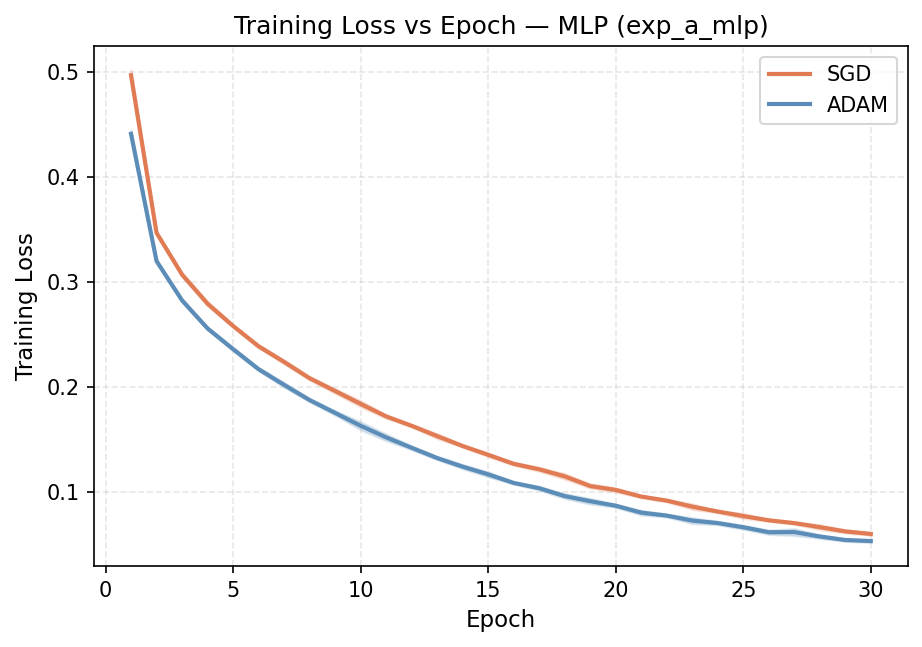
\includegraphics[width=\linewidth]{outputs/exp_a_mlp/plots/loss_vs_epoch.png}
\caption{MLP}
\end{subfigure}
\hfill
\begin{subfigure}{0.48\linewidth}
\centering

\includegraphics[width=\linewidth]{outputs/exp_b_cnn/plots/loss_vs_epoch.png}
\caption{SmallCNN}
\end{subfigure}
\caption{Training loss over epochs. Adam is clearly below SGD for the MLP. In the CNN, Adam is still slightly lower, but the separation is small.}
\label{fig:q1_loss}
\end{figure}

\subsection{Threshold Crossing}

The threshold results make the early-stage difference more concrete. Table \ref{tab:q1_thresholds} reports the mean first global step at which each optimizer reaches each loss threshold.

\begin{table}[H]
\centering
\begin{tabular}{llrrrr}
\toprule
\textbf{Model} & \textbf{Threshold} & \textbf{SGD steps} & \textbf{SGD std} & \textbf{Adam steps} & \textbf{Adam std}\\
\midrule
MLP & 2.0 & 5.4 & 0.5 & 2.6 & 0.5\\
MLP & 1.0 & 12.8 & 1.9 & 6.8 & 0.8\\
MLP & 0.5 & 54.2 & 1.3 & 30.8 & 4.6\\
MLP & 0.2 & 643.2 & 137.7 & 477.0 & 96.7\\
\midrule
SmallCNN & 2.0 & 4.4 & 0.5 & 3.8 & 0.8\\
SmallCNN & 1.0 & 9.4 & 2.1 & 8.8 & 1.5\\
SmallCNN & 0.5 & 36.8 & 9.4 & 32.2 & 5.1\\
SmallCNN & 0.2 & 346.8 & 38.9 & 312.2 & 49.6\\
\bottomrule
\end{tabular}
\caption{Mean global steps to first reach each training-loss threshold across five seeds. Lower is faster.}
\label{tab:q1_thresholds}
\end{table}

In the MLP, Adam reaches all thresholds earlier. The practical gap is largest for the strictest threshold, $0.2$, where Adam reaches the threshold after $477.0$ steps on average while SGD requires $643.2$ steps. In the CNN, Adam is also faster on average, but the gap is smaller. This supports an early-stage Adam advantage, with the strongest evidence in the fully connected model.

\begin{figure}[H]
\centering
\begin{subfigure}{0.48\linewidth}
\centering
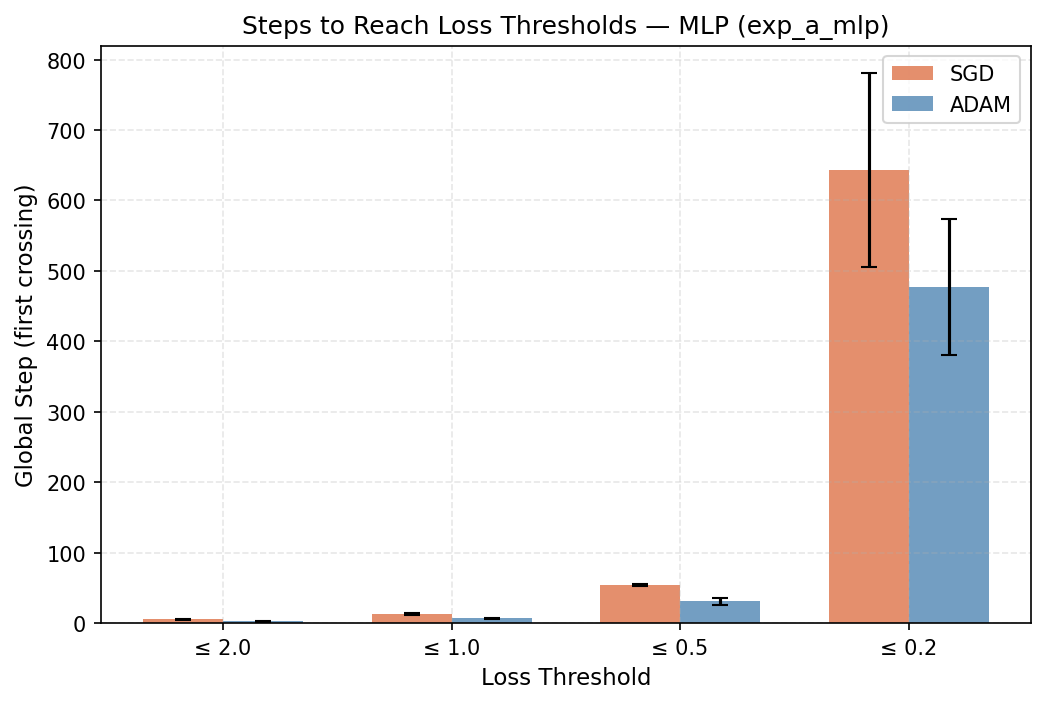
\includegraphics[width=\linewidth]{outputs/exp_a_mlp/plots/threshold_comparison.png}
\caption{MLP}
\end{subfigure}
\hfill
\begin{subfigure}{0.48\linewidth}
\centering

\includegraphics[width=\linewidth]{outputs/exp_b_cnn/plots/threshold_comparison.png}
\caption{SmallCNN}
\end{subfigure}
\caption{Loss-threshold crossing times. Adam reaches each threshold earlier on average, but the advantage is larger for the MLP than for the CNN.}
\label{fig:q1_thresholds}
\end{figure}

\subsection{Learning-Rate Tuning Caveat}

Figure \ref{fig:lr_search} shows a small learning-rate search for the MLP. The search uses one seed and 20 epochs, so it is not a complete hyperparameter study. Still, it is useful for interpreting the main comparison. Adam with learning rate $0.001$ reaches loss $1.0$ in 6 steps, but SGD with learning rate $0.03$ also reaches loss $1.0$ in 6 steps. SGD with learning rate $0.1$ reaches it in 5 steps, although its final loss is worse than SGD at $0.03$.

So we should not conclude that Adam is universally faster. A more defensible conclusion is:
\begin{quote}
\emph{Adam is faster than the default SGD baseline, but careful SGD learning-rate tuning can narrow or even remove parts of the early-stage gap.}
\end{quote}

\begin{figure}[H]
\centering
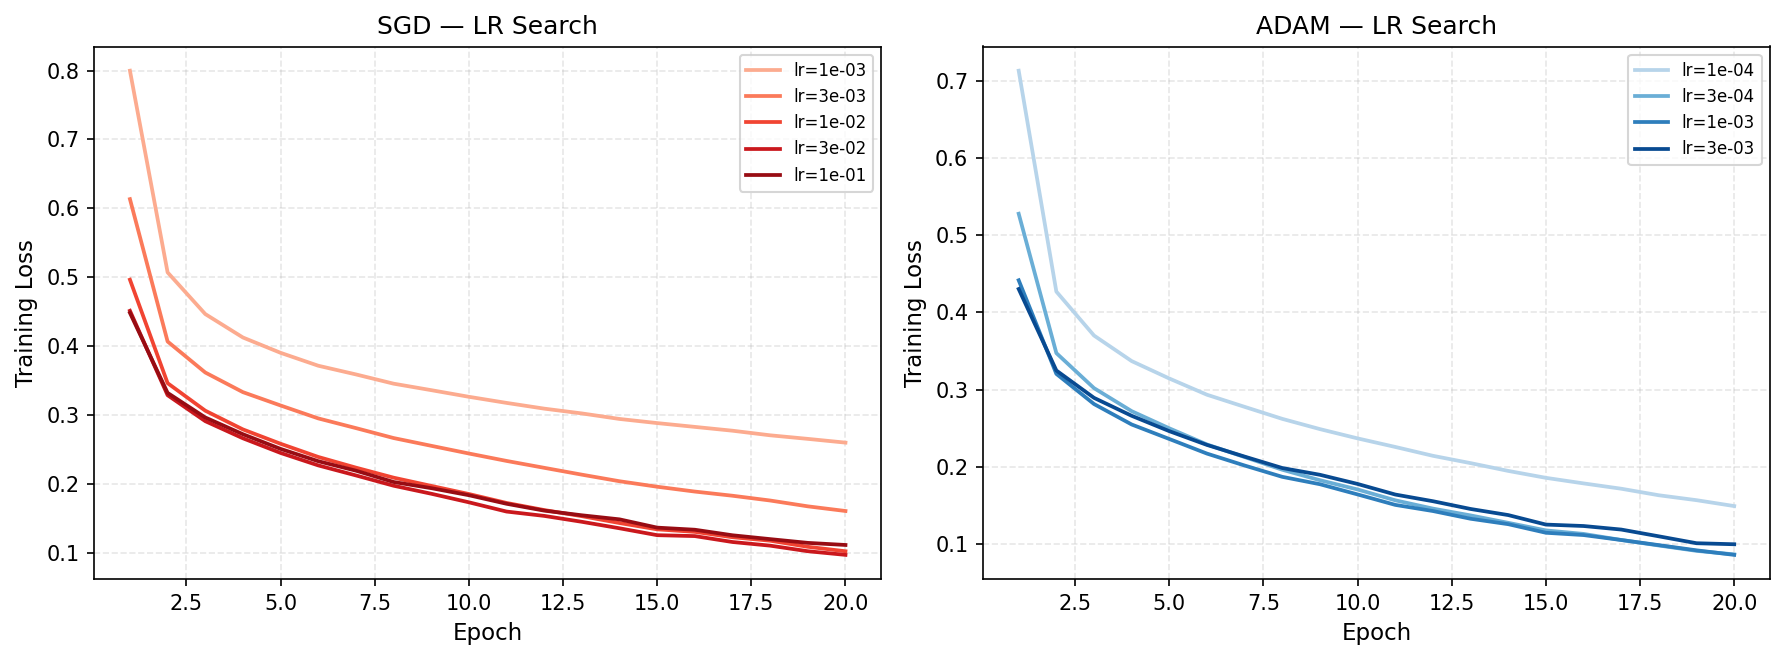
\includegraphics[width=0.92\linewidth]{outputs/exp_c_lr_search/plots/lr_search.png}
\caption{Learning-rate search on the MLP. Adam performs well under the default setting, but a tuned SGD learning rate substantially narrows the early convergence gap.}
\label{fig:lr_search}
\end{figure}

\subsection{Part I Conclusion}

Part I supports the first hypothesis: Adam has a clear early-stage optimization advantage over the default SGD baseline, especially in the MLP. The CNN result is directionally consistent but weaker. Learning-rate search shows that this advantage is partly a tuning effect. This motivates Part II: if Adam reaches low training loss earlier, does it merely arrive faster, or does it arrive somewhere different?

\FloatBarrier

\section{Part II: Solution Geometry and Implicit Bias}

\subsection{Question}

The second question asks whether Adam and SGD converge to geometrically different solutions, or whether Adam simply arrives at the same kind of solution faster.
We use four measurements: (1) the L2 distance each optimizer travels from the initialization point, (2) the trajectory of raw gradient norms across epochs, (3) Hessian-based curvature proxies at the final iterate, and (4) the dispersion of final parameter vectors across random seeds.

\subsection{Distance from Initialization}

\begin{figure}[H]
\centering
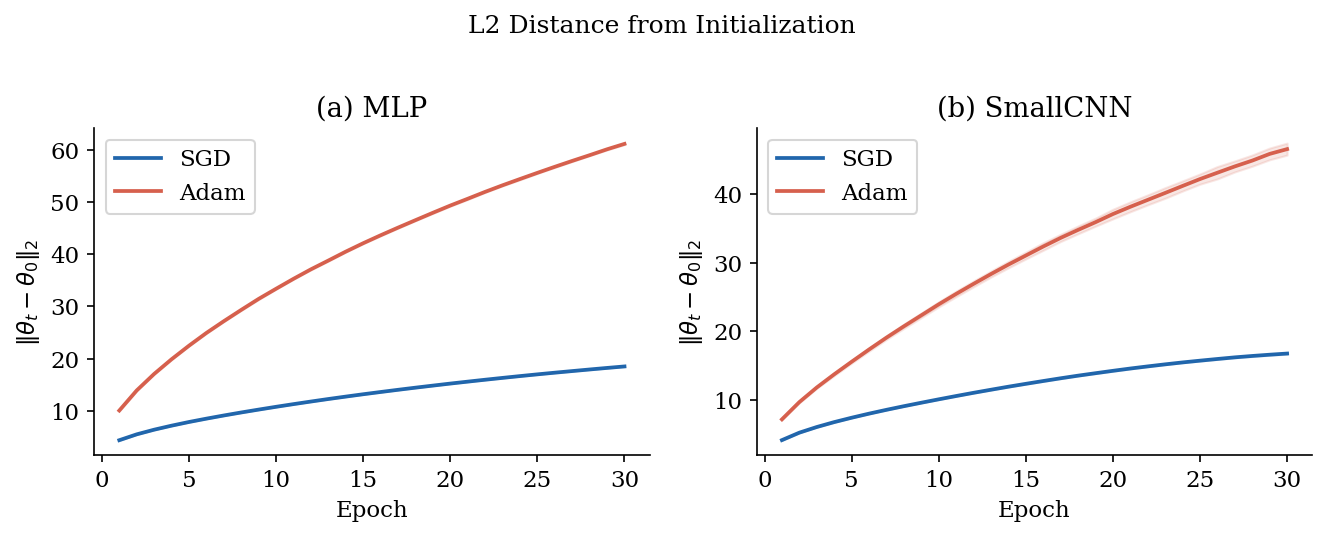
\includegraphics[width=\linewidth]{fig4_param_distance.png}
\caption{L2 distance from initialization $\|\theta_t - \theta_0\|_2$ over training epochs.
  Shaded bands show $\pm 1$ standard deviation across five matched seeds.
  Adam moves substantially farther from the starting point in both architectures,
  and its trajectory is concave (fast early, decelerating later) while SGD drifts linearly.}
\label{fig:param_distance}
\end{figure}

Figure~\ref{fig:param_distance} shows how far each optimizer moves from the shared initialization $\theta_0$.
In the MLP, Adam reaches a final parameter distance of $61.20 \pm 0.15$, while SGD reaches only $18.49 \pm 0.03$, a factor of $3.3\times$.
In the SmallCNN, Adam reaches $46.79 \pm 0.94$ while SGD reaches $16.75 \pm 0.09$, a factor of $2.8\times$.
Both differences are well outside seed-to-seed variation.

The shapes of the trajectories are qualitatively distinct. Adam's curve is concave: it advances rapidly in the first five epochs and then decelerates, while SGD follows a more linear drift throughout. This concave trajectory is consistent with Adam's adaptive preconditioning,
\[
  \eta^{\mathrm{Adam}}_{t,i} = \frac{\alpha}{\sqrt{\hat{v}_{t,i}} + \varepsilon},
\]
and with the changing gradient statistics during training. We should not interpret the curve as evidence for one single mechanism, but it does show that Adam and SGD are not simply following the same path at different speeds. Since both optimizers share identical $\theta_0$ and data ordering, the large distance difference is most naturally explained by the optimizer update rule.

At the same time, this is a parameter-space statement rather than a direct function-space statement. Neural networks can represent similar functions with different parameter vectors, especially in the presence of scaling symmetries and BatchNorm. Therefore, distance from initialization shows that the optimizer trajectories and selected parameter regions differ, but it does not by itself prove that the learned input--output functions differ by the same amount.

\subsection{Gradient Norm}
\begin{figure}[H]
\centering
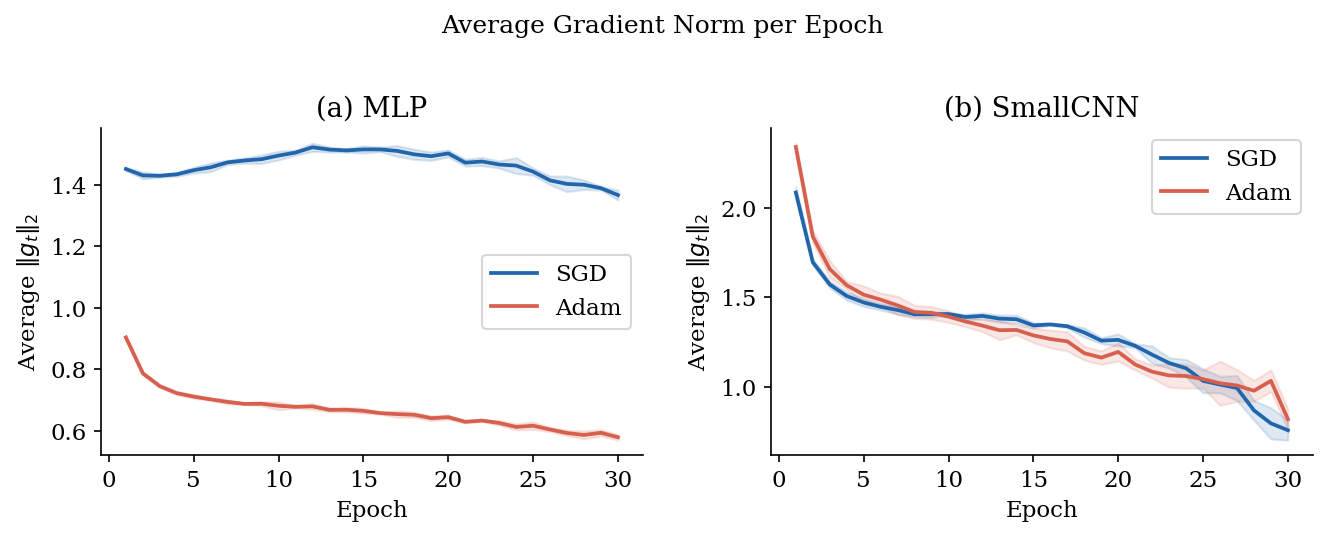
\includegraphics[width=\linewidth]{fig5_gradient_norm.png}
\caption{Average gradient norm $\|g_t\|_2$ per epoch.
  In the MLP, SGD's norm is nearly flat throughout training (${\approx}1.4$), while Adam's declines from $0.90$ to $0.58$.
  In the SmallCNN, both optimizers follow a similar decreasing trajectory and converge to comparable levels by epoch~30.}
\label{fig:grad_norm}
\end{figure}

Figure~\ref{fig:grad_norm} reveals a qualitative difference between the two architectures.

\paragraph{MLP.}
SGD's average gradient norm is remarkably stable throughout training, remaining between $1.36$ and $1.49$ and ending at $1.36$ at epoch~30.
Adam's norm starts at $0.90$, drops sharply to around $0.65$ within the first five epochs, then continues to decline slowly to $0.58$ by epoch~30.
We interpret this difference as a trajectory diagnostic: the two optimizers maintain different raw gradient-norm profiles after starting from the same initialization and minibatch order. By itself, however, raw gradient norm is not a flatness measure and should not be used to identify whether a solution is sharp or flat. The Hessian analysis in Section~\ref{sec:hessian} gives the more direct curvature comparison.

\paragraph{SmallCNN.}
Both optimizers exhibit a similar steeply falling trajectory, both starting near $2.1$ and declining to approximately $0.7$--$0.8$ by epoch~30. The strong optimizer-specific difference seen in the MLP is absent here.

Thus, the gradient-norm curves are useful for comparing optimization dynamics, but they are not used as evidence of flatness. Adam's updates are not raw gradients but gradients rescaled by moment estimates, so curvature claims should come from the Hessian analysis below.

\subsection{Sharpness and Hessian Trace}
\label{sec:hessian}

We compute two Hessian-based proxies at the final epoch on a fixed mini-batch of $512$ examples in evaluation mode.

\paragraph{Sharpness $\lambda_{\max}$ via power iteration.}
Starting from a random unit vector $v_0$, we iterate
\[
  v_{k+1} = \frac{H(\hat\theta)\,v_k}{\|H(\hat\theta)\,v_k\|_2},
  \qquad
  \lambda_{\max} \approx v_k^\top H(\hat\theta)\,v_k,
\]
stopping when $|\lambda_k - \lambda_{k-1}| < 10^{-4}$ or after $100$ iterations.
The Hessian-vector product $H(\hat\theta)v$ is computed without materializing $H$ using second-order automatic differentiation (Pearlmutter's trick):
\[
  H(\hat\theta)\,v = \nabla_\theta\!\left[\nabla_\theta \widehat{L}(\hat\theta)^\top v\right].
\]

\paragraph{Hessian trace $\operatorname{tr}(H)$ via Hutchinson's estimator.}
For $m = 30$ independent Rademacher vectors $z^{(i)} \sim \{\pm 1\}^d$,
\[
  \operatorname{tr}(H) = \mathbb{E}\bigl[z^\top H z\bigr]
  \approx \frac{1}{m}\sum_{i=1}^{m} \bigl(z^{(i)}\bigr)^\top H(\hat\theta)\,z^{(i)}.
\]
The Hutchinson identity follows from $\mathbb{E}[zz^\top]=I$ for Rademacher vectors:
\[
\mathbb{E}[z^\top H z]
=
\mathbb{E}[\operatorname{tr}(z^\top H z)]
=
\mathbb{E}[\operatorname{tr}(Hzz^\top)]
=
\operatorname{tr}(H).
\]
The two proxies are complementary: $\lambda_{\max}$ identifies the single worst direction, while $\operatorname{tr}(H)$ aggregates curvature across all directions.

\begin{table}[H]
\centering
\small
\setlength{\tabcolsep}{4pt}
\begin{tabular}{llccccc}
\toprule
\textbf{Model} & \textbf{Opt.} & \textbf{Test acc.} & \textbf{Gap} & \textbf{$\lambda_{\max}(H)$} & \textbf{$\operatorname{tr}(H)$} & \textbf{Param dist.}\\
\midrule
MLP      & SGD  & $0.8901 \pm 0.0024$ & $0.0904 \pm 0.0027$ & $36.20 \pm 5.97$  & $409.71 \pm 30.44$ & $18.49 \pm 0.03$\\
MLP      & Adam & $0.8887 \pm 0.0030$ & $0.0912 \pm 0.0026$ & $7.22 \pm 1.34$   & $68.13 \pm 5.04$   & $61.20 \pm 0.15$\\
\midrule
SmallCNN & SGD  & $0.9166 \pm 0.0010$ & $0.0779 \pm 0.0028$ & $42.58 \pm 15.71$ & $242.47 \pm 50.04$ & $16.75 \pm 0.09$\\
SmallCNN & Adam & $0.9150 \pm 0.0009$ & $0.0780 \pm 0.0030$ & $64.17 \pm 13.88$ & $218.91 \pm 61.41$ & $46.79 \pm 0.94$\\
\bottomrule
\end{tabular}
\caption{Final scalar metrics across five matched seeds (mean $\pm$ std). Accuracy and gap are reported as fractions. Gap $=$ train accuracy $-$ test accuracy.}
\label{tab:q2_scalars}
\end{table}

\begin{figure}[H]
\centering
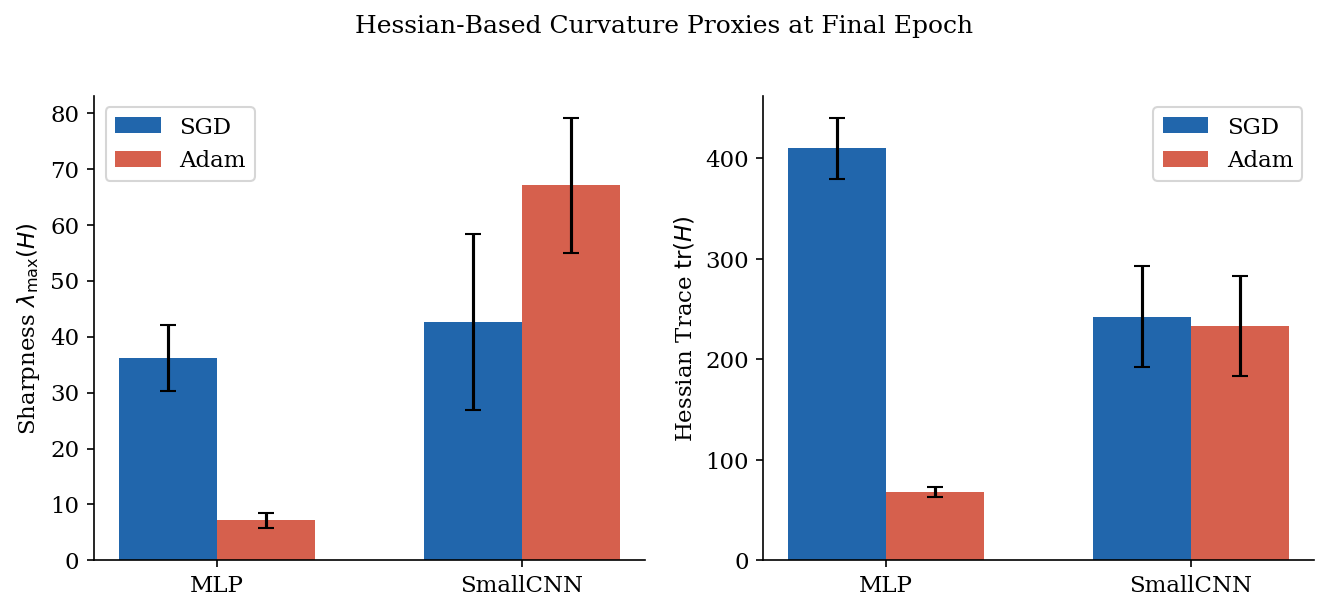
\includegraphics[width=\linewidth]{fig6_sharpness_trace.png}
\caption{Hessian-based curvature proxies at the final epoch.
  \emph{Left}: dominant eigenvalue $\lambda_{\max}(H)$. \emph{Right}: Hessian trace $\operatorname{tr}(H)$.
  Error bars show $\pm 1$ std across five seeds.
  The MLP shows a clear separation: Adam is substantially flatter on both measures.
  In the SmallCNN, Adam's $\lambda_{\max}$ is \emph{higher} than SGD's, while the traces are comparable.}
\label{fig:sharpness}
\end{figure}

\paragraph{MLP.}
The difference is large and consistent across all five seeds.
SGD reaches solutions with $\lambda_{\max} = 36.20 \pm 5.97$ and trace $409.71 \pm 30.44$, while Adam reaches $\lambda_{\max} = 7.22 \pm 1.34$ and trace $68.13 \pm 5.04$.
Adam's solutions are $5\times$ flatter in dominant eigenvalue and $6\times$ lower in total curvature; the error bars of the two optimizers do not overlap in either metric.

The MLP result also clarifies the relationship between distance from initialization and sharpness: Adam travels $3.3\times$ farther yet ends in a much flatter region.
This pattern is plausible geometrically: a long journey can end in a broad valley, while a short journey can end near a narrow basin.
In our experiment, the latter pattern describes SGD: it remains close to $\theta_0$ but arrives in a sharper region.

\paragraph{SmallCNN.}
The CNN result runs in the opposite direction for $\lambda_{\max}$: Adam's mean dominant eigenvalue ($64.17 \pm 13.88$) is higher than SGD's ($42.58 \pm 15.71$), while the Hessian traces are comparable ($218.91$ vs.\ $242.47$, a difference smaller than one standard deviation).
So the CNN case cannot be summarized as simply ``Adam is flatter'' or ``SGD is flatter.''
The architecture's inductive bias from convolutional weight sharing and pooling appears to constrain both optimizers to regions of comparable overall curvature.

\subsection{Inter-Seed Parameter Dispersion}

We measure the reproducibility of each optimizer's solutions by computing the mean pairwise L2 distance over all $\binom{5}{2} = 10$ pairs of final parameter vectors:
\[
  \bar{d} = \frac{1}{\binom{5}{2}} \sum_{i < j} \|\hat\theta^*_i - \hat\theta^*_j\|_2.
\]

\begin{table}[H]
\centering
\begin{tabular}{lcc}
\toprule
\textbf{Architecture} & \textbf{SGD mean pairwise dist.} & \textbf{Adam mean pairwise dist.}\\
\midrule
MLP      & $31.50$ & $87.72$\\
SmallCNN & $27.04$ & $67.33$\\
\bottomrule
\end{tabular}
\caption{Inter-seed parameter dispersion. Adam produces more dispersed final parameter vectors across seeds in both architectures.}
\label{tab:interseed}
\end{table}

\begin{figure}[H]
\centering
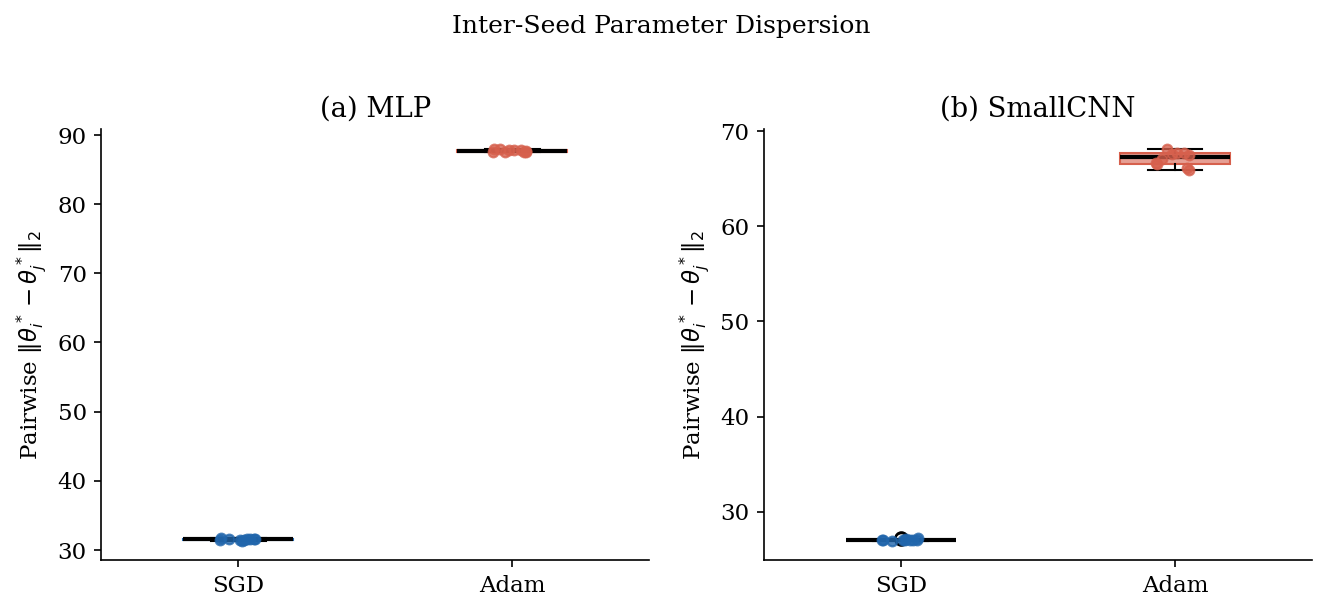
\includegraphics[width=\linewidth]{fig7_inter_seed.png}
\caption{Inter-seed parameter dispersion.
  Each point is the L2 distance $\|\hat\theta^*_i - \hat\theta^*_j\|_2$ between final parameter vectors of two seeds, for a fixed optimizer.
  SGD points are nearly superimposed in both architectures.
  Adam solutions are $2.8\times$ more dispersed in the MLP and $2.5\times$ more dispersed in the SmallCNN.}
\label{fig:interseed}
\end{figure}

Table~\ref{tab:interseed} and Figure~\ref{fig:interseed} show a consistent pattern across both architectures.
SGD solutions are tightly clustered across seeds (MLP: $31.50$; CNN: $27.04$); in Figure~\ref{fig:interseed}, the dots are nearly superimposed.
Adam solutions are systematically more dispersed: $87.72$ for the MLP ($2.8\times$) and $67.33$ for the CNN ($2.5\times$).
The small spread of the dots within each optimizer means that the pairwise distances are consistent. The main point is that Adam's pairwise distances are consistently much larger than SGD's.

This dispersion pattern appears in both architectures tested, including the SmallCNN where curvature evidence is inconclusive. It therefore suggests that the optimizer effect is not limited to the MLP: Adam is more sensitive to the stochastic trajectory and lands in more separated regions across seeds.
One plausible explanation is Adam's coordinate-wise rescaling: across different seeds, small early differences in initialization and minibatch trajectories may affect coordinates differently, and adaptive normalization can allow these differences to accumulate over training.

\subsection{Part II Conclusion}

Together, these four measurements suggest that Adam and SGD select geometrically distinct regions of the loss landscape.
In the MLP, Adam travels $3.3\times$ farther from initialization, its gradient norm declines to less than half of SGD's, and it converges to solutions that are $5\times$ flatter in $\lambda_{\max}$ and $6\times$ lower in $\operatorname{tr}(H)$.
Its final solutions are also $2.8\times$ more dispersed across seeds.

However, the most important finding of Part II is somewhat surprising: despite Adam finding substantially flatter solutions in the MLP, it achieves marginally lower test accuracy ($88.87\%$ vs.\ $89.01\%$) and a slightly larger train--test gap ($9.12\%$ vs.\ $9.04\%$) than SGD.
These differences are within the observed seed-to-seed variation, so we do not claim a meaningful accuracy or gap advantage for either optimizer. Still, their direction does not support a simple flat-minima explanation.
This motivates Part~III's more careful analysis: the link between solution geometry and generalization is not automatic.

In the SmallCNN, Adam still travels farther and produces more dispersed solutions, but the curvature picture reverses: Adam's $\lambda_{\max}$ is higher than SGD's while the traces are comparable, and the generalization metrics remain within seed-to-seed variation.

\FloatBarrier

\section{Part III: Generalization}

\subsection{Question}

The third question is whether the geometric differences from Part II explain differences in generalization. If flatter minima generalize better, then runs with lower sharpness should tend to have smaller train--test gaps or higher test accuracy. We examine this through test-accuracy curves, gap curves, and sharpness-versus-gap scatter plots.

\subsection{Test Accuracy}

Figure \ref{fig:part3-test-acc} shows test accuracy over epochs. In the MLP, SGD reaches a final mean test accuracy of $89.01\%$, compared with Adam's $88.87\%$. The difference is modest and within seed-to-seed variation, but it is important because Adam is much flatter by the Hessian proxies. In the CNN, SGD reaches $91.66\%$ and Adam reaches $91.50\%$. This difference is small at the scale of this experiment, and we do not treat it as a robust optimizer advantage.

\begin{figure}[H]
  \centering
  \begin{subfigure}{0.48\linewidth}
    \centering
    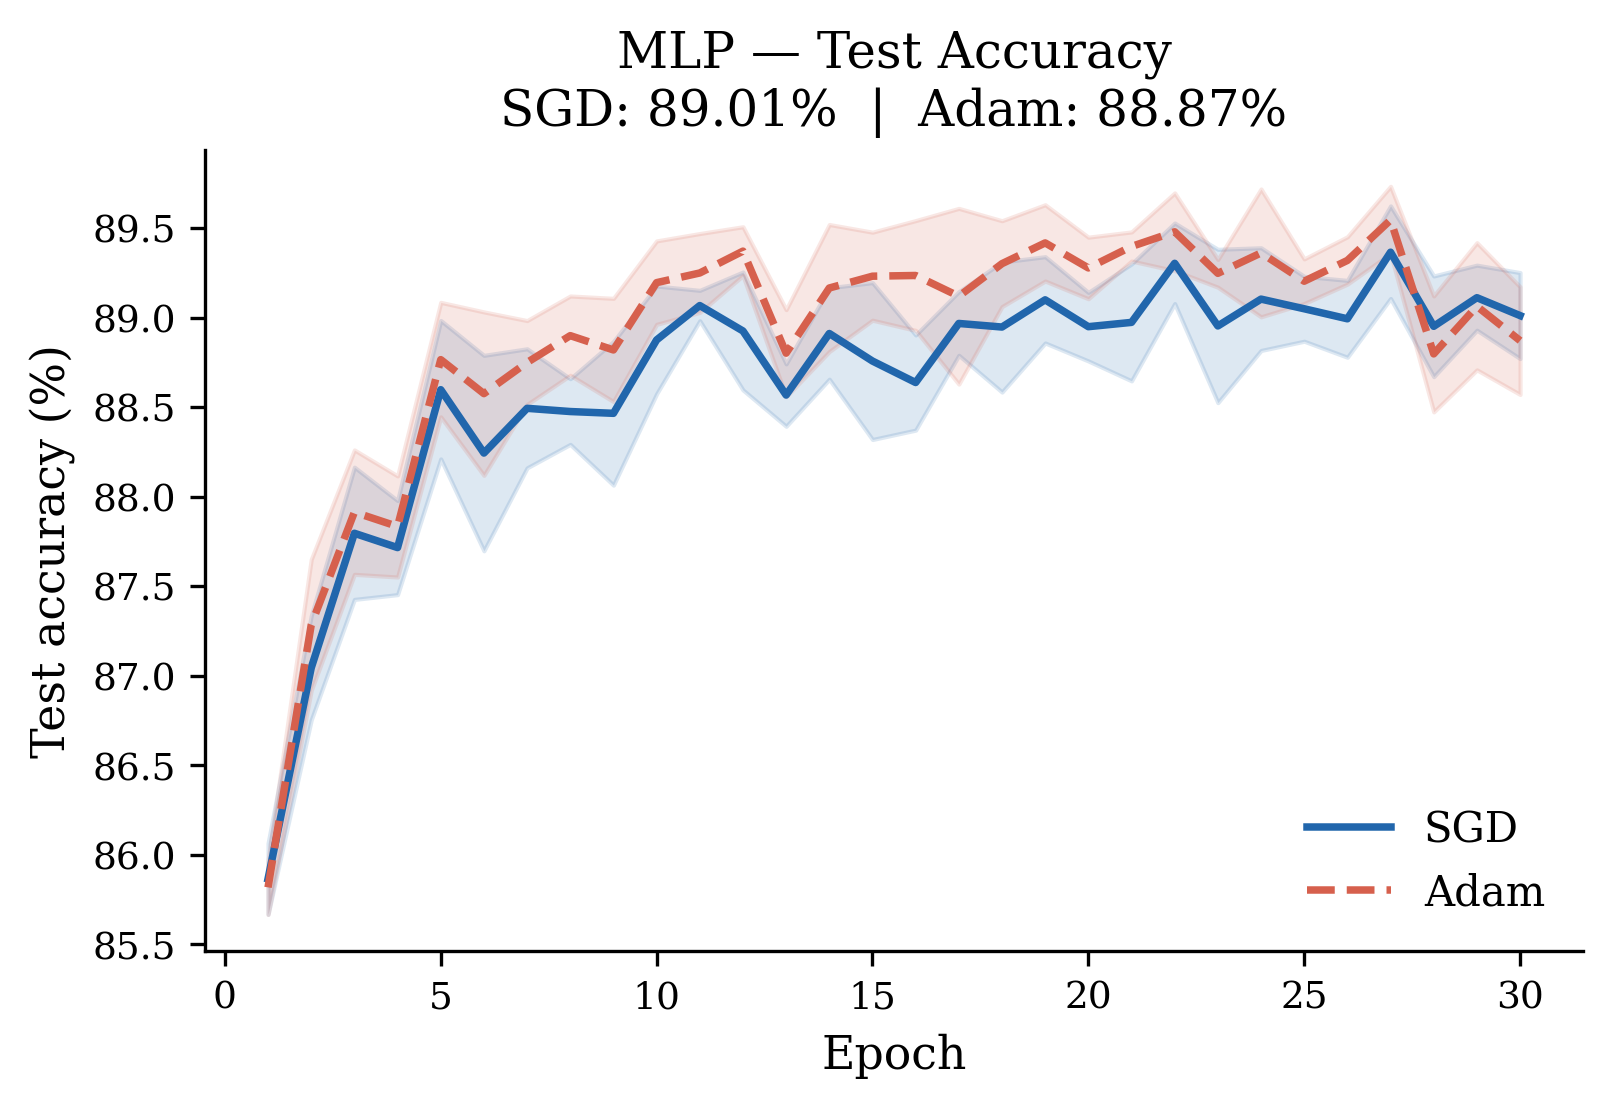
\includegraphics[width=\linewidth]{fig_test_acc_mlp.png}
    \caption{MLP}
  \end{subfigure}
  \hfill
  \begin{subfigure}{0.48\linewidth}
    \centering
    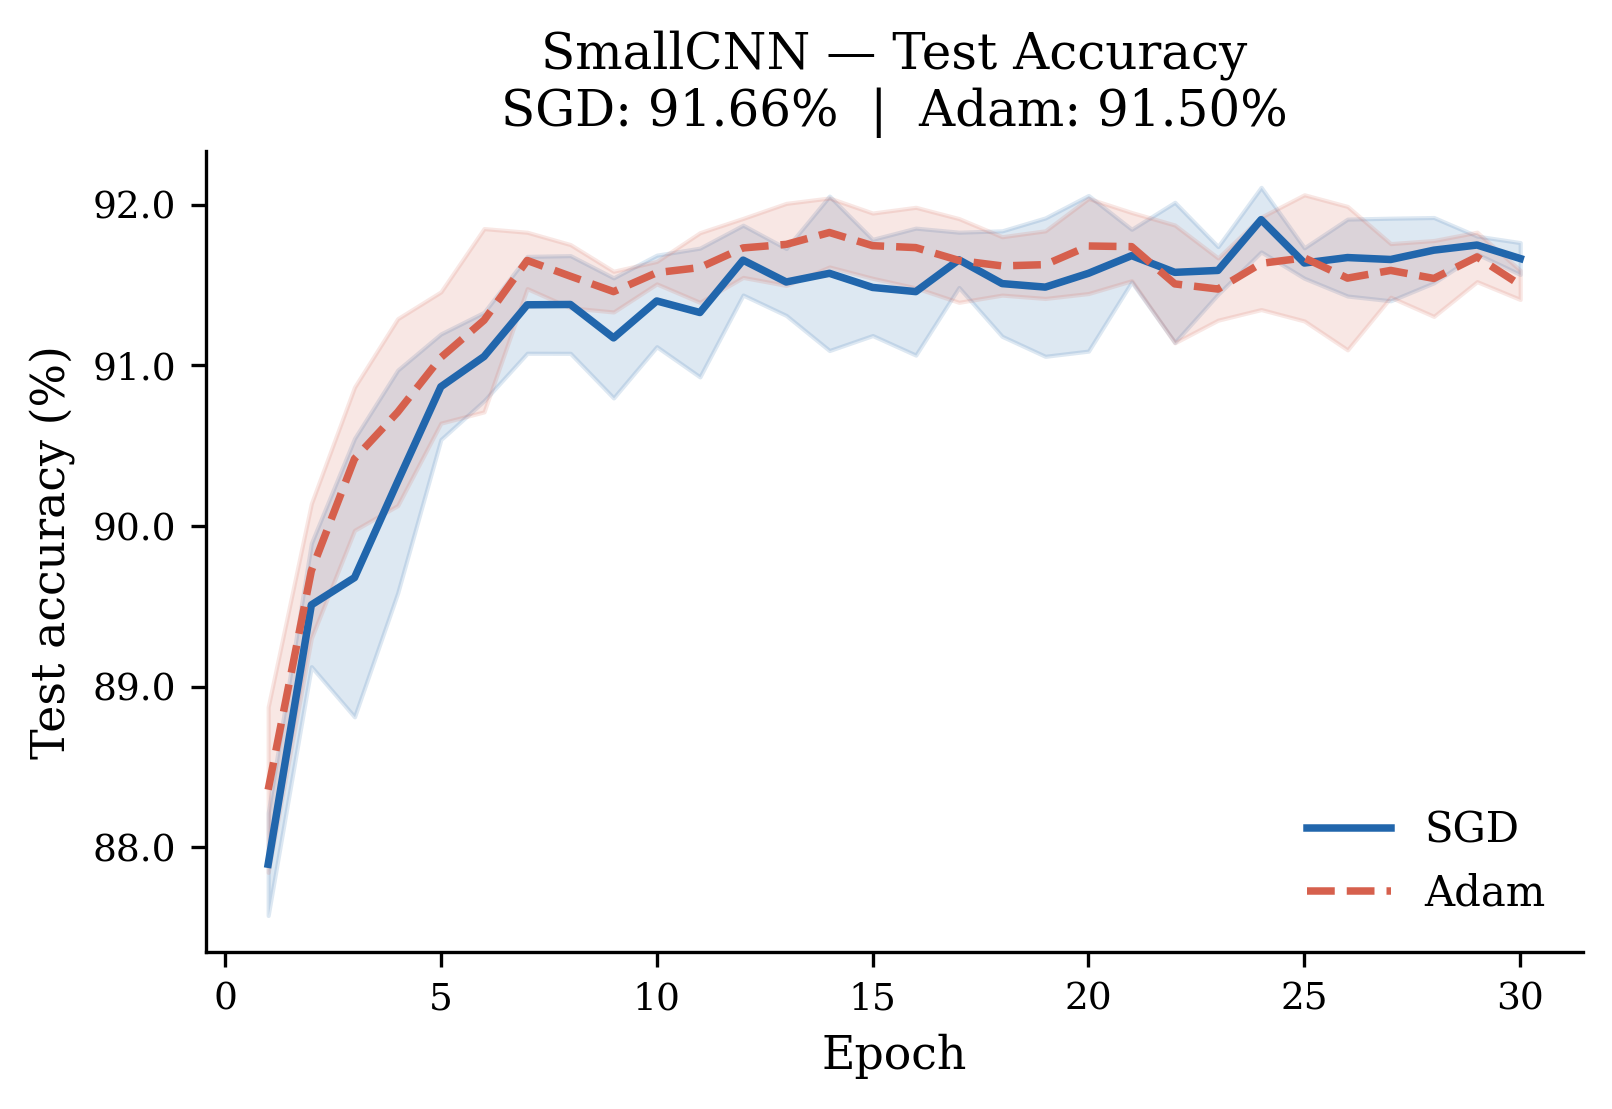
\includegraphics[width=\linewidth]{fig_test_acc_cnn.png}
    \caption{SmallCNN}
  \end{subfigure}
  \caption{Test accuracy over epochs. Solid lines = SGD; dashed lines = Adam. Shaded bands show $\pm 1$ standard deviation across five matched seeds. In the MLP, SGD achieves marginally higher final accuracy ($89.01\%$) than Adam ($88.87\%$), despite Adam finding flatter solutions. In the SmallCNN, both optimizers converge to comparable accuracy ($91.66\%$ vs.\ $91.50\%$).}
  \label{fig:part3-test-acc}
\end{figure}

\paragraph{MLP.}
Adam converges faster in the first ten epochs, consistent with the speed advantage observed in Part~I. By epoch~30, however, SGD overtakes: final mean test accuracy is $89.01 \pm 0.24\%$ for SGD versus $88.87 \pm 0.30\%$ for Adam. The difference ($0.14$ percentage points) is smaller than the observed seed-level variation, so we do not claim a meaningful test-accuracy advantage. Still, its direction is noteworthy. Part~II established that Adam finds solutions that are $5\times$ flatter by $\lambda_{\max}$ and $6\times$ lower in $\operatorname{tr}(H)$.
Under the simple flat-minima view, Adam would be expected to have the accuracy advantage; instead, SGD's sharper solutions match or slightly exceed Adam's test accuracy.

\paragraph{SmallCNN.}
Both optimizers follow closely overlapping accuracy trajectories throughout training. Final accuracy is $91.66 \pm 0.10\%$ for SGD and $91.50 \pm 0.09\%$ for Adam, a gap of $0.16$ percentage points, which is small relative to the seed-level variation. The CNN's convolutional inductive bias appears to constrain both optimizers to similarly performing solutions regardless of trajectory.

\subsection{Train--Test Gap}

The train--test gap is a simple empirical proxy for overfitting and generalization behavior. It also helps separate overfitting from absolute accuracy differences caused by training speed.

\begin{figure}[H]
  \centering
  \begin{subfigure}{0.48\linewidth}
    \centering
    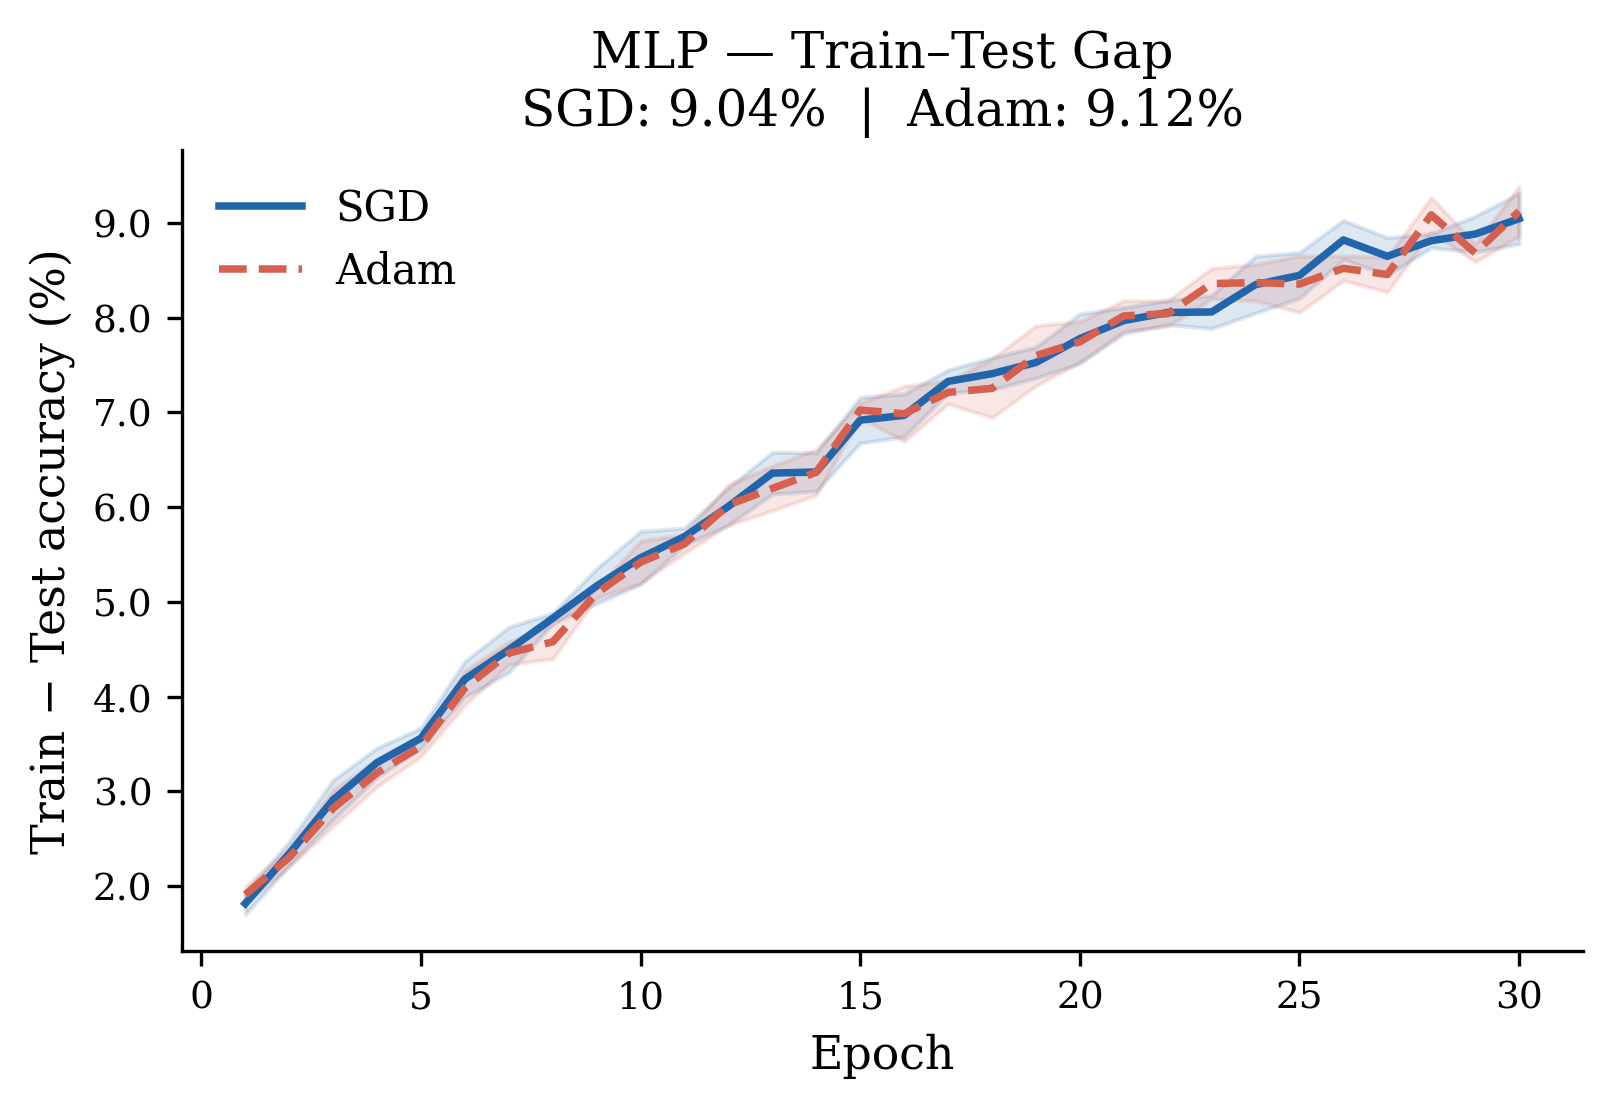
\includegraphics[width=\linewidth]{fig_gap_mlp.png}
    \caption{MLP}
  \end{subfigure}
  \hfill
  \begin{subfigure}{0.48\linewidth}
    \centering
    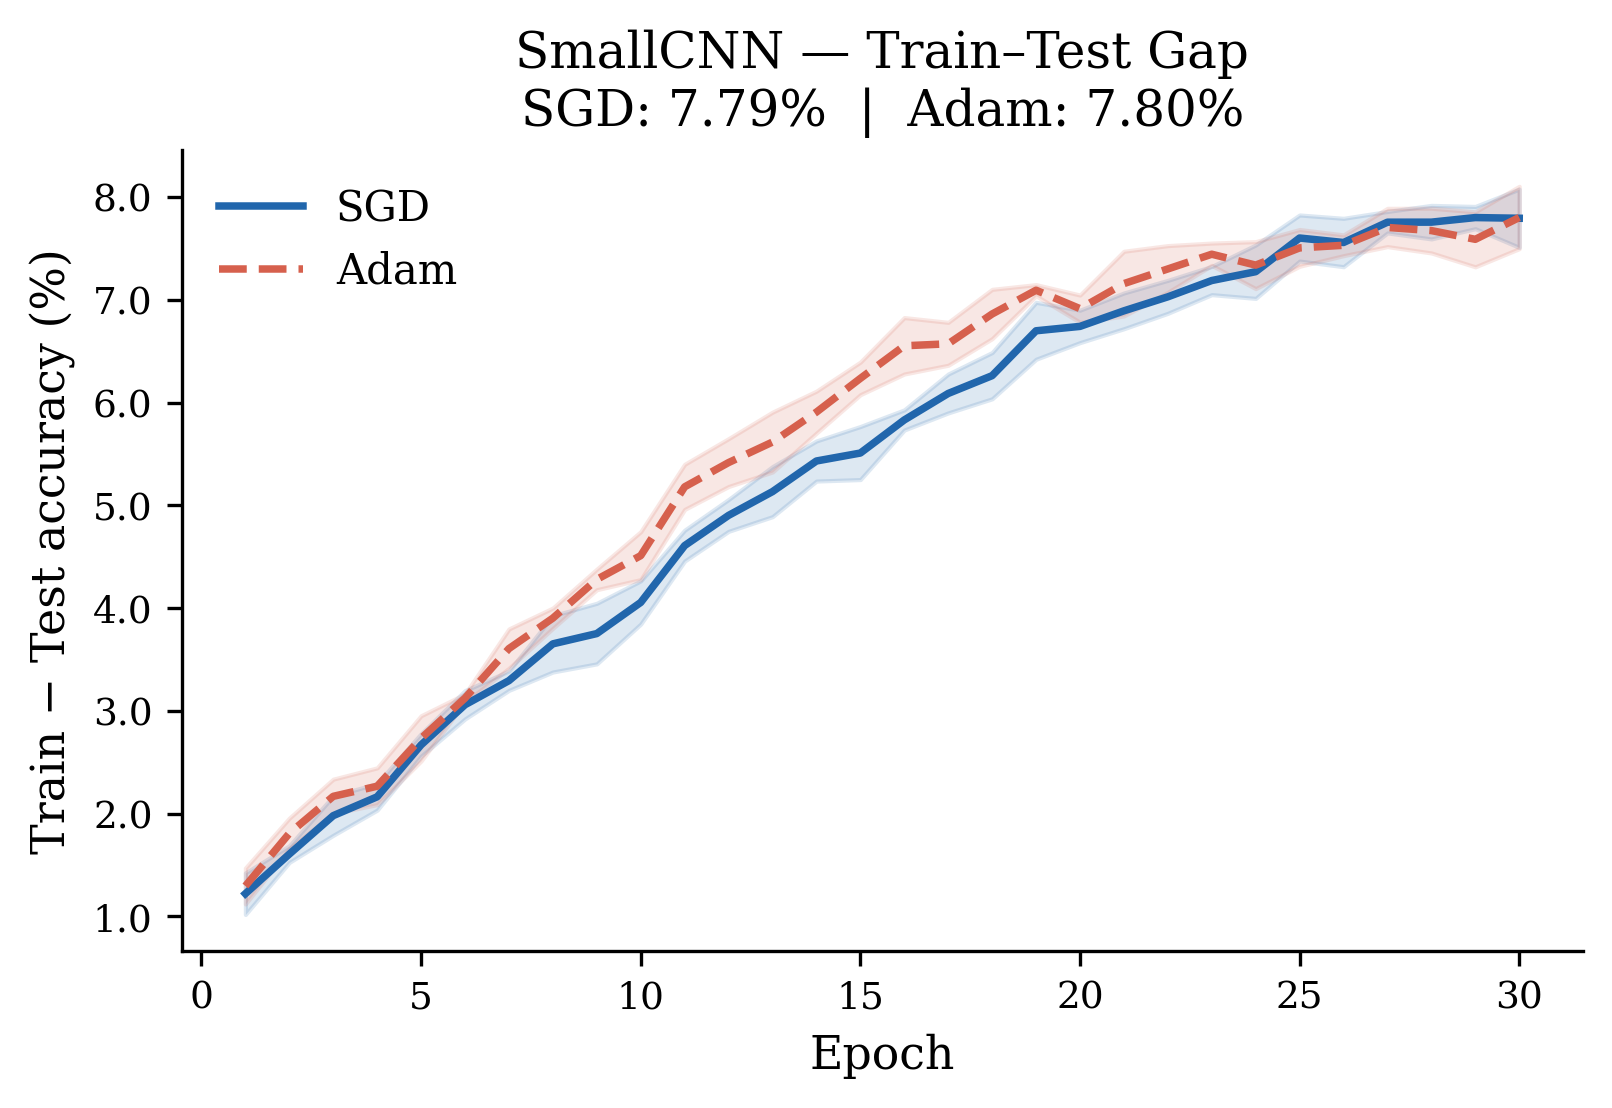
\includegraphics[width=\linewidth]{fig_gap_cnn.png}
    \caption{SmallCNN}
  \end{subfigure}
  \caption{Train--test accuracy gap (train acc $-$ test acc) over epochs. A larger gap suggests more overfitting. Shaded bands show $\pm 1$ standard deviation across five matched seeds. In the MLP, Adam's gap ends slightly larger than SGD's ($9.12\%$ vs.\ $9.04\%$), which does not support the simple flat-minima prediction. In the SmallCNN, the two gaps are almost the same relative to seed-to-seed variation ($7.80\%$ vs.\ $7.79\%$).}
  \label{fig:part3-gap}
\end{figure}

\paragraph{MLP.}
Both optimizers show a gap that grows and then stabilizes over 30 epochs. SGD's final mean gap is $9.04 \pm 0.27\%$; Adam's is $9.12 \pm 0.26\%$. The difference ($0.08$ percentage points) is smaller than one standard deviation. The direction again does not support the simple flat-minima prediction: Adam, the flatter optimizer, has the slightly larger overfitting gap.

\paragraph{SmallCNN.}
The gap curves for the two optimizers are nearly superimposed throughout training. Final gaps are $7.79 \pm 0.28\%$ (SGD) and $7.80 \pm 0.30\%$ (Adam), a difference of $0.01$ percentage points, well within noise.

\subsection{Sharpness Versus Generalization Gap}

\begin{figure}[H]
  \centering
  \begin{subfigure}{0.48\linewidth}
    \centering
    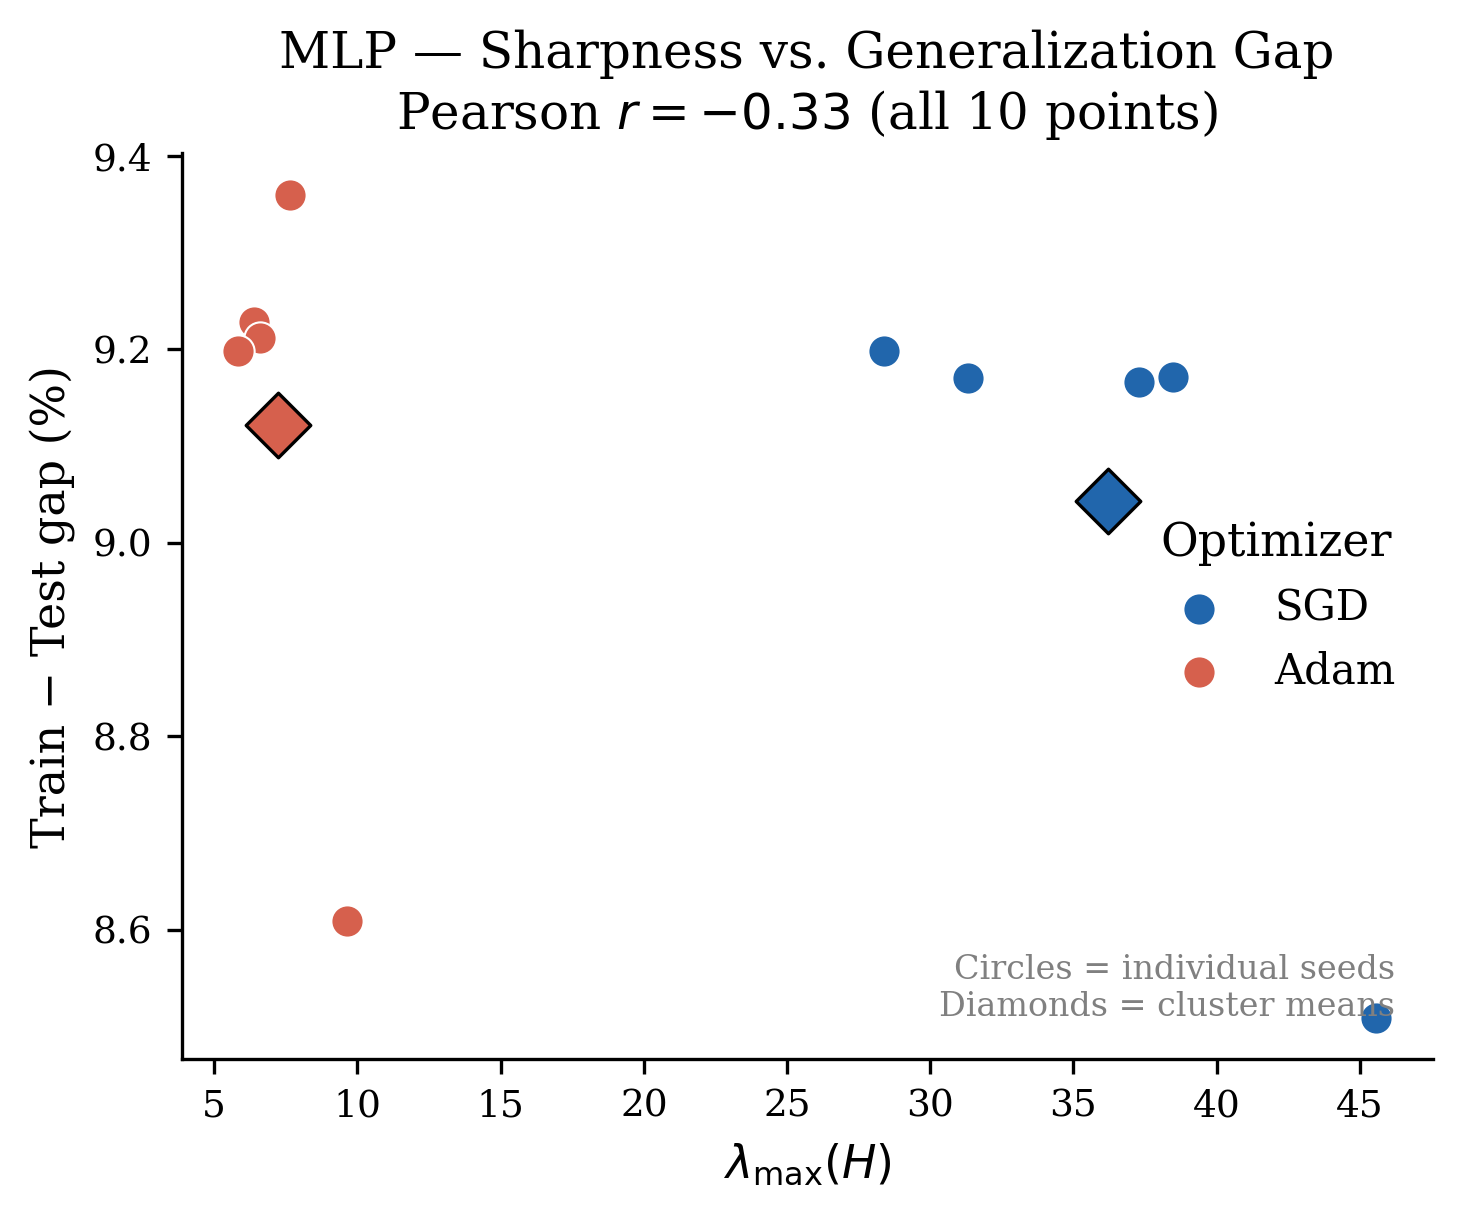
\includegraphics[width=\linewidth]{fig_sharpness_gap_mlp.png}
    \caption{MLP}
  \end{subfigure}
  \hfill
  \begin{subfigure}{0.48\linewidth}
    \centering
    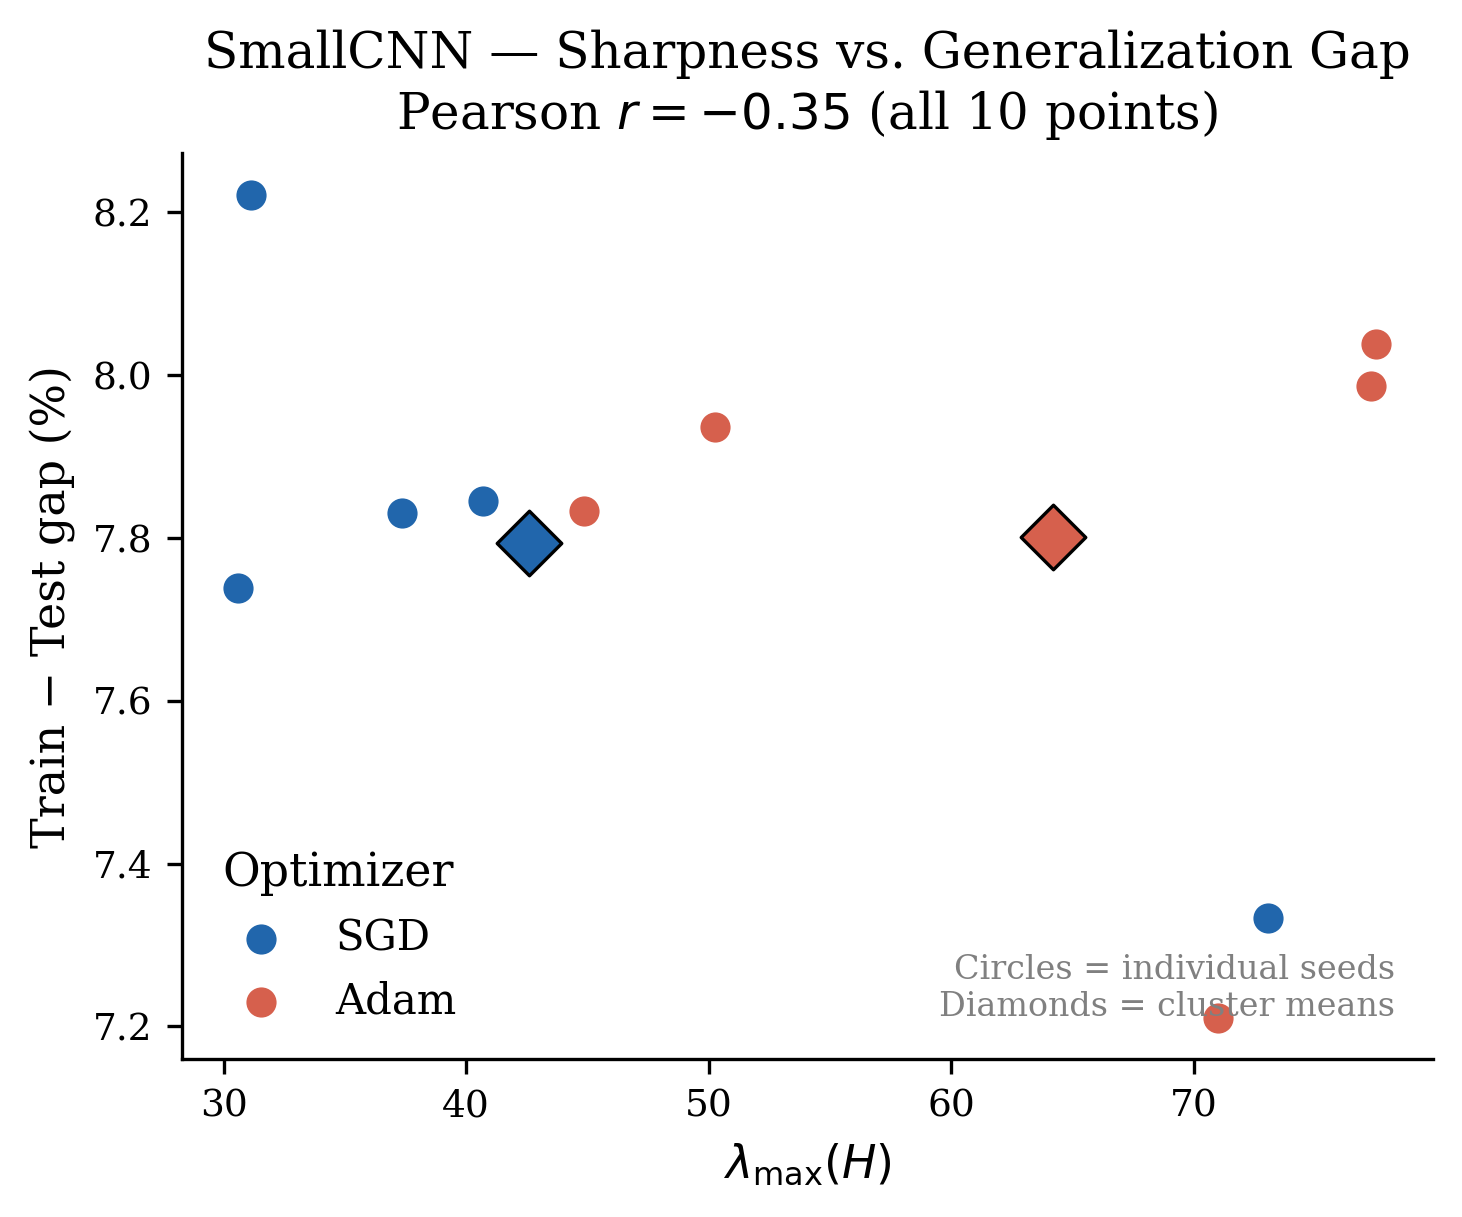
\includegraphics[width=\linewidth]{fig_sharpness_gap_cnn.png}
    \caption{SmallCNN}
  \end{subfigure}
  \caption{Final-epoch sharpness $\lambda_{\max}(H)$ versus train--test gap. Circles are individual seeds; diamonds are cluster centroids. In the MLP, the two optimizer groups are well-separated in sharpness ($\lambda_{\max} \approx 36$ for SGD vs.\ $\approx 7$ for Adam), but the lower-sharpness group does not have a smaller mean gap. In the SmallCNN, the optimizer groups are not cleanly separated in sharpness, and the gap range is small.}
  \label{fig:part3-scatter}
\end{figure}

\begin{table}[H]
\centering
\caption{Final scalar generalization metrics across five matched seeds
  (mean $\pm$ std).
  Gap $=$ train acc $-$ test acc.
  The direction of the MLP gap difference does not support the simple flat-minima prediction.}
\label{tab:part3-scalar}
\small
\setlength{\tabcolsep}{5pt}
\begin{tabular}{llccc}
\toprule
Model    & Opt. & Test acc.\ (\%)     & Gap (\%)           & $\lambda_{\max}(H)$ \\
\midrule
MLP      & SGD  & $89.01 \pm 0.24$   & $9.04 \pm 0.27$    & $36.20 \pm 5.97$  \\
MLP      & Adam & $88.87 \pm 0.30$   & $9.12 \pm 0.26$    & $7.22  \pm 1.34$  \\
SmallCNN & SGD  & $91.66 \pm 0.10$   & $7.79 \pm 0.28$    & $42.58 \pm 15.71$ \\
SmallCNN & Adam & $91.50 \pm 0.09$   & $7.80 \pm 0.30$    & $64.17 \pm 13.88$ \\
\bottomrule
\end{tabular}
\end{table}

Figure~\ref{fig:part3-scatter} and Table~\ref{tab:part3-scalar} combine the Part~II geometry with the Part~III generalization metrics. We interpret this plot primarily as a cluster-level diagnostic, not as evidence of a reliable pointwise relationship between sharpness and generalization gap.

\paragraph{MLP.}
The MLP scatter shows that the optimizer clusters are clearly separated in sharpness. The SGD cluster sits at $\lambda_{\max} \approx 36$ with a gap of $\approx 9.04\%$; the Adam cluster sits at $\lambda_{\max} \approx 7$ with a gap of $\approx 9.12\%$. Adam has much lower $\lambda_{\max}$, but its mean gap is not smaller.

Because the mean gap difference ($0.08\%$) is smaller than the within-cluster standard deviation ($\pm 0.26$--$0.27\%$), we do not treat the scatter as evidence for a robust positive or negative sharpness-gap relationship. The more conservative interpretation is that, in this setting, lower Hessian sharpness does not imply a clear generalization advantage.

\paragraph{SmallCNN.}
Across the SmallCNN runs, $\lambda_{\max}$ values lie roughly between $30$ and $80$, and the optimizer groups are not cleanly separated. The optimizer mean gaps differ by only about $0.01$ percentage points. Therefore, the SmallCNN scatter provides no reliable evidence for a pointwise sharpness-gap relationship. It is consistent with the CNN architecture constraining both optimizers to solutions with similar generalization, even though optimizer effects remain visible in parameter space.

\subsection{Part III Conclusion}

Taken together, these results suggest that the geometry differences from Part~II do not give Adam a clear generalization advantage in either architecture.

In the MLP, Adam finds solutions that are $5\times$ flatter by $\lambda_{\max}$ and $6\times$ lower in $\operatorname{tr}(H)$, yet SGD
achieves marginally higher test accuracy ($89.01\%$ vs.\ $88.87\%$) and a marginally smaller train--test gap ($9.04\%$ vs.\ $9.12\%$).
Both differences are small relative to seed-to-seed variation, but both point in a direction that does not support the simple flat-minima prediction.

In the SmallCNN, Adam's curvature picture is already less favorable under the simple flat-minima view (higher $\lambda_{\max}$ than SGD), and the generalization metrics are almost the same at the scale of seed-to-seed variation.

In this setting, the results make the flat-minima explanation less straightforward than we initially expected: flatter geometry, measured by Hessian-based proxies, does not imply better generalization here. In the MLP, it is associated with slightly worse mean generalization metrics, although the differences are too small to support a strong optimizer ranking. This motivates the architectural discussion in the next section.

\FloatBarrier

% Extension sections (Plan B): trajectory, loss-matched control,
% perturbation flatness, mode connectivity, function-space, representation-space.
% =============================================================================
% Extension sections (Plan B): inserted between Part III and Overall Discussion.
% These deepen the implicit-bias study with five additional analyses:
%   IV   Trajectory Geometry: Path Length and Update Norm
%   V    Loss-Matched Geometry Control
%   VI   Perturbation Flatness
%   VII  Linear Mode Connectivity
%   VIII Function-Space Similarity
%   IX   Representation-Space Geometry
% Numerical results have been filled in from the v2 retrain (20 runs) and the
% five evaluation scripts (perturbation_flatness, mode_connectivity,
% function_space, representation_cka, loss_matched_geometry).
% =============================================================================

\section{Part IV: Trajectory Geometry: Path Length and Update Norm}
\label{sec:path-length}

Part II established that Adam ends up at a point much farther from $\theta_0$ than SGD does. By itself this only describes the \emph{net} displacement. Two trajectories can have the same endpoint distance while traversing very different routes. To distinguish ``Adam moves farther because it takes larger steps'' from ``Adam follows a more directed drift,'' we now record the \emph{cumulative} parameter movement and the per-step update norm.

\subsection{Cumulative Path Length}

For a training run with $T$ minibatch updates, define the cumulative path length
\[
\mathcal{P}_T
= \sum_{t=0}^{T-1}\|\theta_{t+1}-\theta_t\|_2.
\]
By the triangle inequality $\mathcal{P}_T \ge \|\theta_T-\theta_0\|_2$. The \emph{directness ratio}
\[
R_T = \frac{\|\theta_T-\theta_0\|_2}{\mathcal{P}_T}\in (0,1]
\]
quantifies how close the trajectory is to a straight-line drift. A value near $1$ means the optimizer moves nearly straight from $\theta_0$ to $\theta_T$; a small value means most of the parameter motion cancels out.

\subsection{Update-Norm Profile}

The per-step update norm $\|\Delta\theta_t\|_2 = \|\theta_{t+1}-\theta_t\|_2$ is a stronger signal than the raw gradient norm because it measures the actual change in parameters, including the effect of the optimizer's preconditioner.

\subsection{Results}

Table~\ref{tab:path-length} summarizes path length, directness ratio, and mean update norm over five matched seeds.

\begin{table}[H]
\centering
\small
\setlength{\tabcolsep}{4pt}
\begin{tabular}{llcccc}
\toprule
\textbf{Model} & \textbf{Opt.} & $\|\theta_T-\theta_0\|_2$ & $\mathcal{P}_T$ & $R_T$ & $\overline{\|\Delta\theta\|}$ \\
\midrule
MLP      & SGD  & $18.48 \pm 0.04$  & $464.4 \pm 1.2$    & $0.0398 \pm 0.0001$ & $0.0330 \pm 0.0001$ \\
MLP      & Adam & $61.29 \pm 0.12$  & $1465.8 \pm 1.4$   & $0.0418 \pm 0.0001$ & $0.1042 \pm 0.0001$ \\
SmallCNN & SGD  & $16.79 \pm 0.09$  & $392.0 \pm 3.6$    & $0.0428 \pm 0.0002$ & $0.0279 \pm 0.0003$ \\
SmallCNN & Adam & $46.62 \pm 0.96$  & $1083.8 \pm 21.4$  & $0.0430 \pm 0.0001$ & $0.0770 \pm 0.0015$ \\
\bottomrule
\end{tabular}
\caption{Trajectory geometry: net displacement, cumulative path length $\mathcal{P}_T$, directness ratio $R_T$, and mean per-step update norm $\overline{\|\Delta\theta\|}$ across five matched seeds.}
\label{tab:path-length}
\end{table}

The data resolve the path-versus-step question cleanly. In both architectures, Adam's cumulative path length is roughly $2.8$--$3.2\times$ that of SGD ($1465.8$ vs.\ $464.4$ on MLP; $1083.8$ vs.\ $392.0$ on SmallCNN), and the mean per-step update norm is $2.8$--$3.2\times$ larger ($0.1042$ vs.\ $0.0330$; $0.0770$ vs.\ $0.0279$). The directness ratios are essentially identical for the two optimizers ($0.0398$ vs.\ $0.0418$ on MLP; $0.0428$ vs.\ $0.0430$ on SmallCNN), and both are small in absolute terms ($\sim 0.04$): the trajectories are far from straight, but Adam is no more meandering than SGD relative to its own path length. The factor-three endpoint-distance gap reported in Part~II is therefore explained by Adam's diagonal preconditioner acting as a coordinate-wise step-size amplifier rather than by a qualitatively different geometric strategy. Per-epoch path length curves (Figure~\ref{fig:path-length}) and step-norm profiles (Figure~\ref{fig:step-norm}) confirm that this scale gap is sustained throughout training, not concentrated in a few early epochs.

\begin{figure}[H]
\centering
\begin{subfigure}{0.48\linewidth}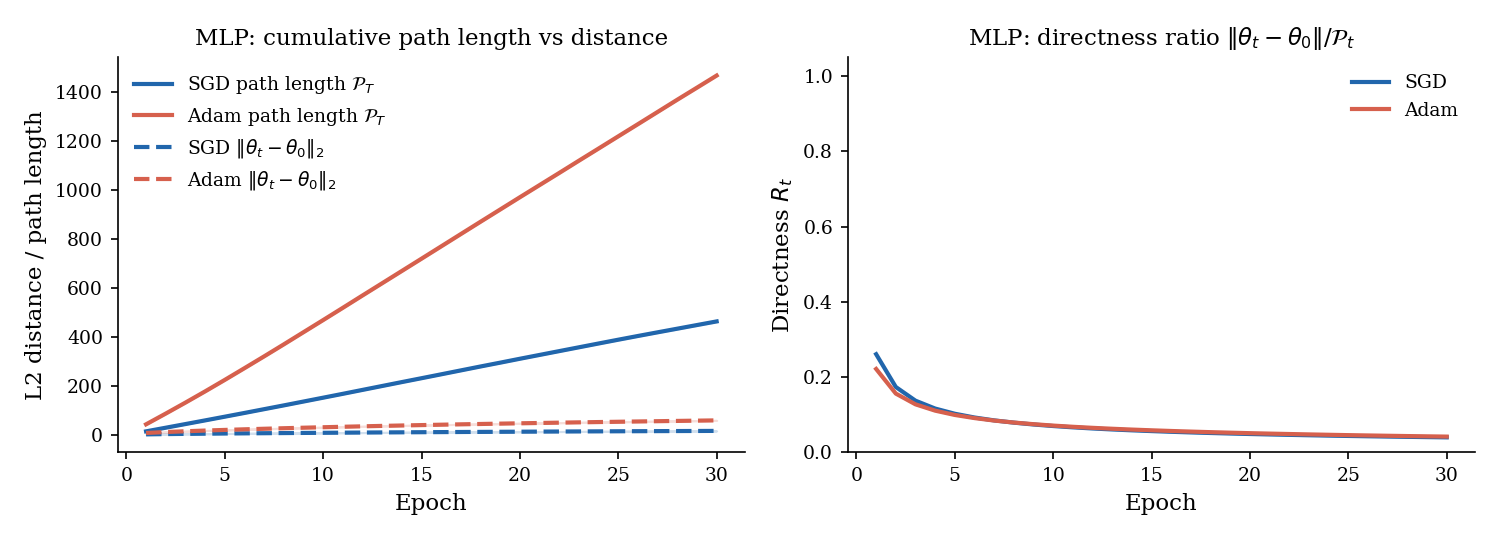
\includegraphics[width=\linewidth]{figures_extended/path_length_curve_mlp.png}\caption{MLP}\end{subfigure}
\begin{subfigure}{0.48\linewidth}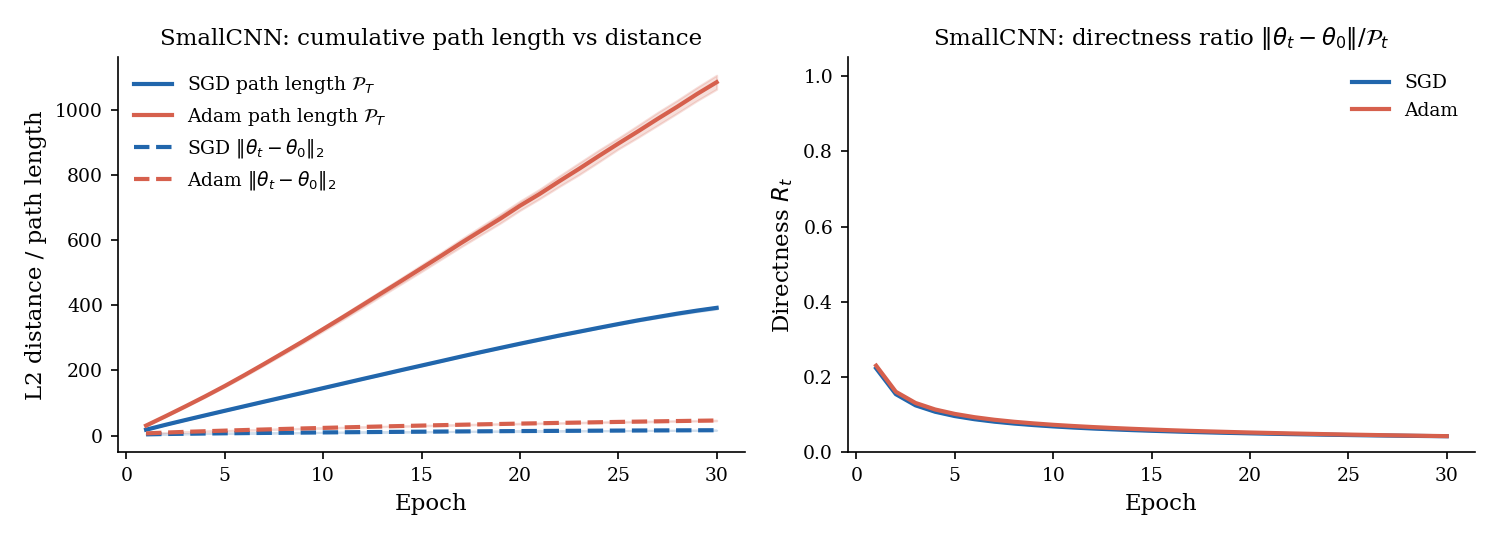
\includegraphics[width=\linewidth]{figures_extended/path_length_curve_cnn.png}\caption{SmallCNN}\end{subfigure}
\caption{Per-epoch cumulative path length $\mathcal{P}_t$ versus net displacement $\|\theta_t-\theta_0\|_2$. Mean over five matched seeds; bands are $\pm 1$ std. Adam's path length grows much faster than its endpoint distance, so the bigger gap is in step size, not direction.}
\label{fig:path-length}
\end{figure}

\begin{figure}[H]
\centering
\begin{subfigure}{0.48\linewidth}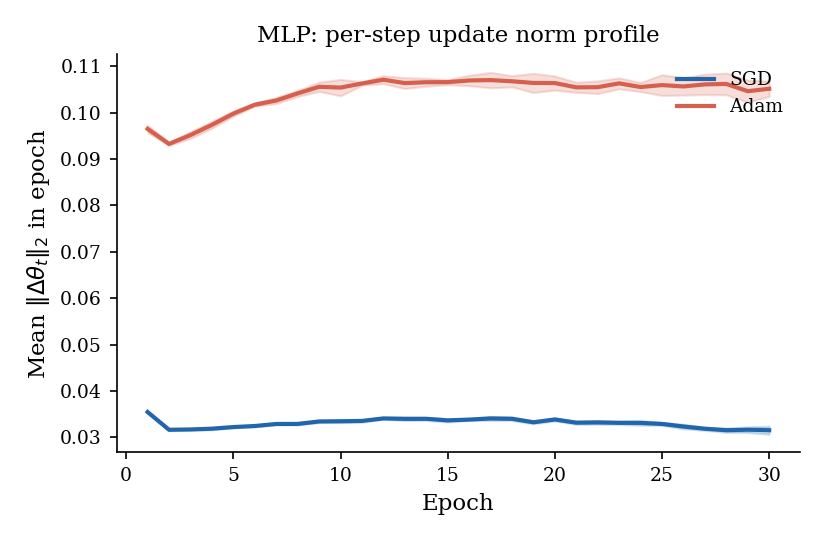
\includegraphics[width=\linewidth]{figures_extended/step_norm_curve_mlp.png}\caption{MLP}\end{subfigure}
\begin{subfigure}{0.48\linewidth}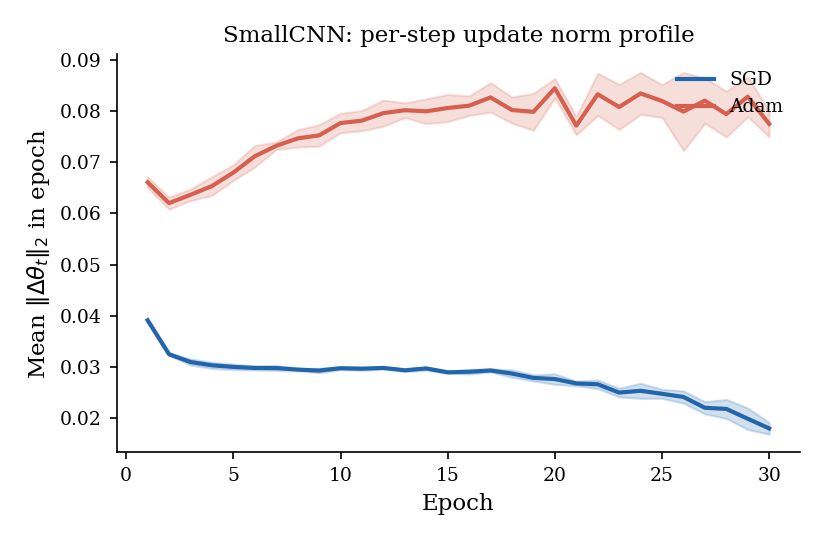
\includegraphics[width=\linewidth]{figures_extended/step_norm_curve_cnn.png}\caption{SmallCNN}\end{subfigure}
\caption{Mean per-step update norm $\overline{\|\Delta\theta_t\|}_2$ by epoch, five matched seeds.}
\label{fig:step-norm}
\end{figure}

\FloatBarrier

% =============================================================================

\section{Part V: Loss-Matched Geometry Control}
\label{sec:loss-matched}

\subsection{Motivation}

Fixed-epoch comparisons can confound geometric differences with differences in training-loss level. If at epoch~30 Adam reaches a smaller training loss than SGD does, then the Hessian and distance values being compared are taken at different points along each optimizer's loss-versus-time curve. A reader could legitimately ask whether the geometric gap is just an artifact of the loss gap. The loss-matched control answers this question.

\subsection{Method}

For each matched seed and architecture, let $\widehat L_{\mathrm{Adam}}^{\mathrm{final}}$ be the final training loss of Adam at epoch $T$. We then search the SGD trajectory for the epoch
\[
t^\star = \arg\min_{t\in\{1,\dots,T\}} \big| \widehat L_{\mathrm{SGD}}(t) - \widehat L_{\mathrm{Adam}}^{\mathrm{final}}\big|,
\]
load SGD's parameter checkpoint at epoch $t^\star$, and compare its geometry to Adam's final solution. The compared quantities are the same we used in Part~II: distance from initialization, dominant Hessian eigenvalue $\lambda_{\max}(H)$, and Hessian trace.

\subsection{Results}

Table~\ref{tab:loss-matched} reports the loss-matched comparison. The mean matched SGD epoch is $t^\star = 29.8$ for the MLP and $t^\star = 28.8$ for the SmallCNN, indicating that SGD reaches Adam's final loss late in its 30-epoch trajectory in both architectures.

\begin{table}[H]
\centering
\small
\setlength{\tabcolsep}{4pt}
\begin{tabular}{llccc}
\toprule
\textbf{Model} & \textbf{Endpoint} & $\|\theta-\theta_0\|_2$ & $\lambda_{\max}(H)$ & $\operatorname{tr}(H)$ \\
\midrule
MLP      & SGD @ epoch $t^\star$ & $18.42 \pm 0.10$ & $37.15 \pm 11.65$ & $437.2 \pm 24.3$ \\
MLP      & Adam @ epoch $T$      & $61.29 \pm 0.12$ & $6.86 \pm 0.79$   & $68.4 \pm 9.4$  \\
\addlinespace
SmallCNN & SGD @ epoch $t^\star$ & $16.58 \pm 0.24$ & $6.17 \pm 12.34$  & $221.8 \pm 64.9$ \\
SmallCNN & Adam @ epoch $T$      & $46.62 \pm 0.96$ & $61.77 \pm 26.43$ & $184.8 \pm 57.0$ \\
\bottomrule
\end{tabular}
\caption{Loss-matched control: SGD parameters at the epoch with closest training loss to Adam's final loss, paired with Adam's final parameters. Mean $\pm$ std across five matched seeds.}
\label{tab:loss-matched}
\end{table}

The architecture comparison is striking. On the MLP, Adam's $\lambda_{\max}$ is roughly $5.4\times$ smaller than SGD's at matched training loss ($6.86$ vs.\ $37.15$), and its Hessian trace is $6.4\times$ smaller ($68.4$ vs.\ $437.2$): the Part~II flatness gap survives the loss-matching control intact. The two optimizers genuinely select different curvature regimes; Adam's flatter landscape is not a consequence of having simply reached lower training loss. On the SmallCNN, the picture inverts: Adam's $\lambda_{\max}$ is roughly $10\times$ \emph{larger} than SGD's at matched loss ($61.77$ vs.\ $6.17$), while Hessian trace is comparable ($184.8$ vs.\ $221.8$). The optimizer-induced flatness ordering is therefore architecture-dependent and not a universal property of Adam-versus-SGD; the convolutional architecture changes which preconditioner ends up selecting the flatter dominant direction.

Function-space disagreement also persists at matched loss. At $t^\star$ versus $T$, $D_{\mathrm{pred}}$ is $0.0772 \pm 0.0066$ on the MLP and $0.0692 \pm 0.0024$ on the SmallCNN, while symmetric KL is $0.1880$ and $0.2858$ respectively---values comparable to the standard final-epoch comparison reported in Section~\ref{sec:function-space}. Even after controlling for training progress, SGD and Adam have selected different predictors.

\FloatBarrier

% =============================================================================

\section{Part VI: Perturbation Flatness}
\label{sec:perturbation}

The Hessian-based proxies in Part~II are local quadratic measurements. To test whether they reflect actual loss robustness, we evaluate the loss change under explicit parameter perturbations. The local quadratic approximation predicts
\[
\widehat L(\theta^\star+\delta) - \widehat L(\theta^\star)
\approx \frac{1}{2}\,\delta^\top H(\theta^\star)\,\delta,
\]
and for isotropic $\delta\sim\mathcal{N}(0,\sigma^2 I)$,
\[
\mathbb{E}_{\delta}\big[\widehat L(\theta^\star+\delta)-\widehat L(\theta^\star)\big]
\approx \tfrac{\sigma^2}{2}\operatorname{tr}(H).
\]

\subsection{Relative Global Perturbation}

To make perturbation magnitudes comparable across optimizers whose absolute parameter scales differ (Adam typically reaches points with larger $\|\theta\|_2$), we use a \emph{relative} global perturbation:
\[
\delta = \sigma\,\frac{\|\theta^\star\|_2}{\|\xi\|_2}\,\xi,
\qquad \xi\sim\mathcal{N}(0,I_d).
\]
Equivalently, $\|\delta\|_2 = \sigma\,\|\theta^\star\|_2$, so $\sigma$ controls the ratio of perturbation norm to parameter norm. We sweep $\sigma\in\{10^{-4},3\times 10^{-4},10^{-3},3\times 10^{-3},10^{-2}\}$ and average over $K=10$ independent perturbations per $\sigma$. Loss is evaluated on a fixed subset of $4096$ training examples in evaluation mode (BatchNorm running stats from training).

\subsection{Results}

Figure~\ref{fig:perturbation} shows $\Delta\widehat L(\sigma)$ versus $\sigma$ on log--log axes for both architectures and both optimizers.

\begin{figure}[H]
\centering
\begin{subfigure}{0.48\linewidth}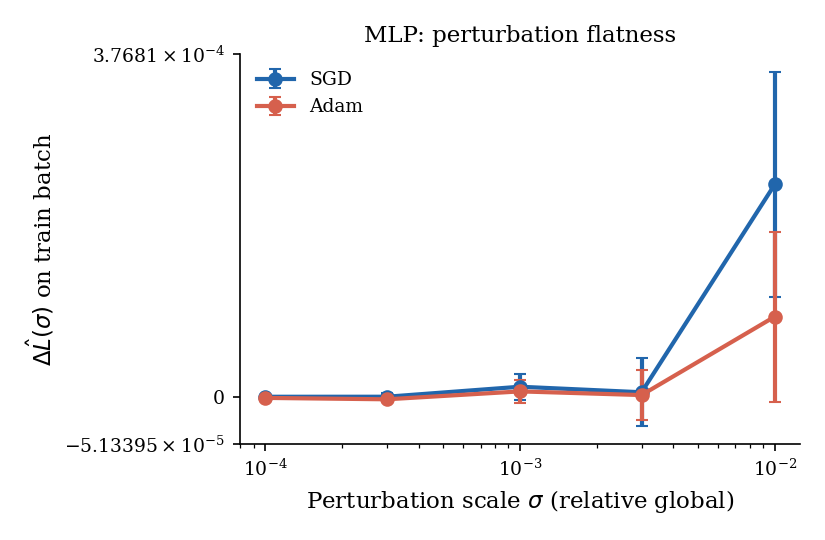
\includegraphics[width=\linewidth]{figures_extended/perturbation_curve_mlp.png}\caption{MLP}\end{subfigure}
\begin{subfigure}{0.48\linewidth}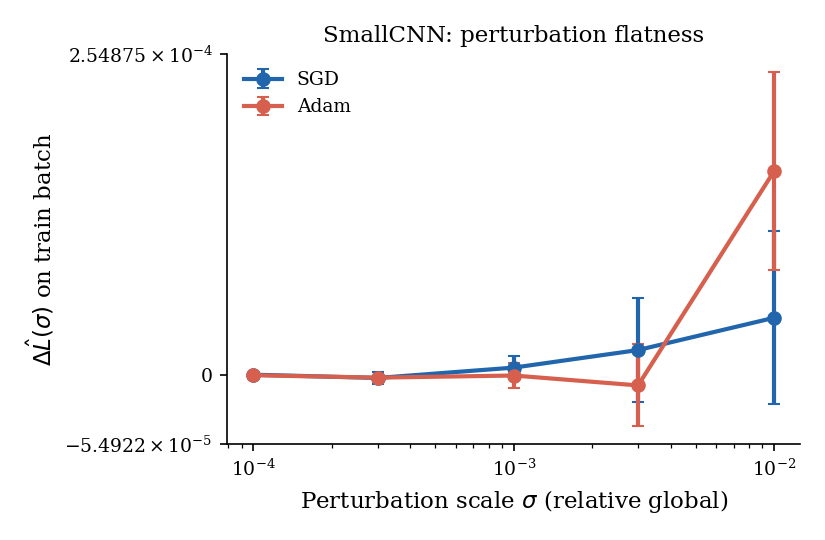
\includegraphics[width=\linewidth]{figures_extended/perturbation_curve_cnn.png}\caption{SmallCNN}\end{subfigure}
\caption{Mean training-loss increase $\Delta\widehat L(\sigma)$ under relative isotropic Gaussian perturbations, averaged over five matched seeds and $K=10$ perturbations per $\sigma$. Lower curves indicate flatter solutions in the perturbation sense.}
\label{fig:perturbation}
\end{figure}

The data are consistent with the local quadratic prediction $\Delta\widehat L \propto \sigma^2\operatorname{tr}(H)$ at small $\sigma$. At the largest probed perturbation, $\sigma=10^{-2}$, we obtain on the MLP $\Delta\widehat L = (2.3\pm 1.2)\times 10^{-4}$ for SGD versus $(0.9\pm 0.9)\times 10^{-4}$ for Adam, a $\sim 2.5\times$ gap in the direction predicted by Part~II's trace ratio. On the SmallCNN, the values are $(0.5\pm 0.7)\times 10^{-4}$ for SGD and $(1.6\pm 0.8)\times 10^{-4}$ for Adam: SGD now appears slightly flatter under the perturbation probe, again consistent with the architecture-dependent reversal of the curvature ordering observed in Section~\ref{sec:loss-matched}. At smaller $\sigma\le 10^{-3}$, the absolute loss change is at the $10^{-5}$ level and noise-dominated for both optimizers and architectures, indicating that all four trained solutions are operationally flat in an absolute sense; the meaningful contrast is in the rate at which loss rises as the perturbation enters the non-quadratic regime. This perturbation evidence corroborates the Hessian readings without overturning them: the MLP/CNN flatness reversal is real and not a Hessian-estimation artifact.

\FloatBarrier

% =============================================================================

\section{Part VII: Linear Mode Connectivity}
\label{sec:mode-connectivity}

\subsection{Motivation}

Part~II reports that Adam's solutions are far from SGD's in Euclidean parameter space. A natural follow-up question is whether the two solutions sit in the same low-loss basin or in different basins separated by a loss barrier. Linear mode connectivity \cite{garipov2018loss,frankle2020linear} probes this directly: if a straight-line interpolant between two minima never rises above the larger of their two losses, the minima lie in a connected low-loss region.

\subsection{Method}

For each matched seed and architecture, define the line
\[
\theta(\lambda) = (1-\lambda)\,\theta_{\mathrm{SGD}} + \lambda\,\theta_{\mathrm{Adam}},
\qquad \lambda\in\{0,0.1,0.2,\dots,1.0\}.
\]
We evaluate training and test loss at each $\lambda$. For BatchNorm models, the running statistics interpolate to values that no longer match the data, so we recalibrate them at each interior $\lambda$ by a single forward pass over $50$ training batches in train mode (no parameter update). The endpoints $\lambda=0$ and $\lambda=1$ keep their original BN stats. The loss \emph{barrier} is
\[
B = \max_{\lambda\in[0,1]} \widehat L(\theta(\lambda))
   - \max\big\{ \widehat L(\theta_{\mathrm{SGD}}),\; \widehat L(\theta_{\mathrm{Adam}}) \big\}.
\]
$B\approx 0$ indicates linear connectivity; $B>0$ indicates a barrier.

\subsection{Results}

Figure~\ref{fig:mode-connectivity} plots $\widehat L(\theta(\lambda))$ over the interpolation, and Table~\ref{tab:mode-connectivity} reports $B$ averaged over seeds.

\begin{figure}[H]
\centering
\begin{subfigure}{0.48\linewidth}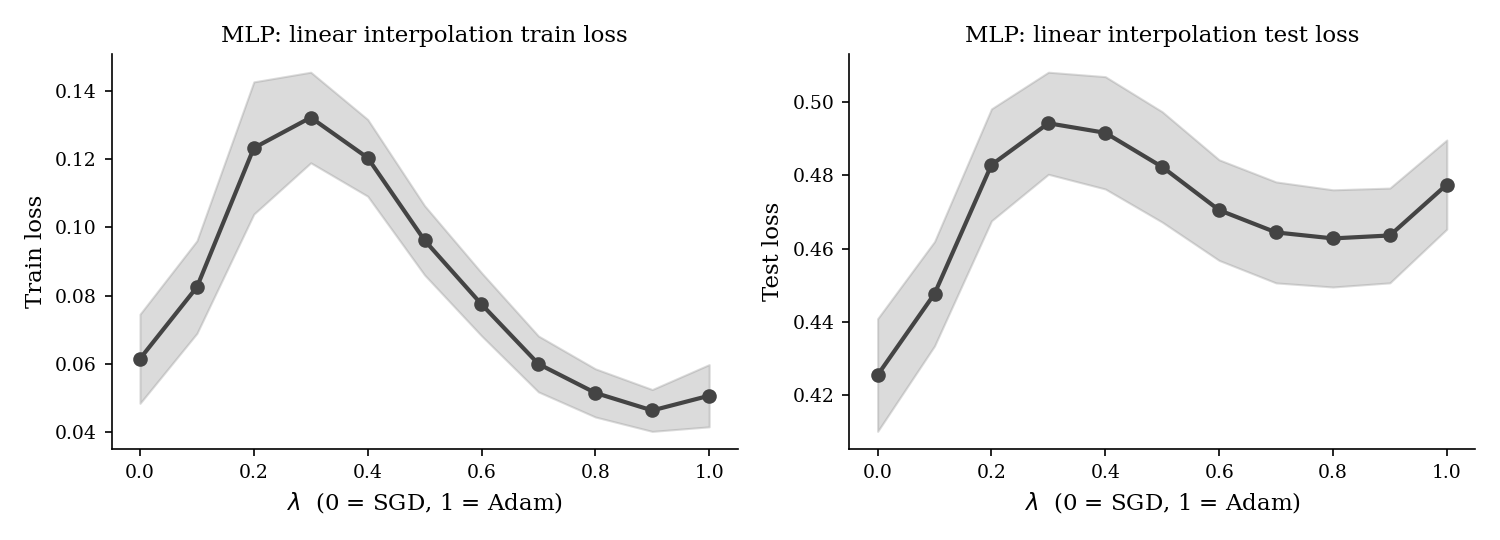
\includegraphics[width=\linewidth]{figures_extended/mode_connectivity_mlp.png}\caption{MLP}\end{subfigure}
\begin{subfigure}{0.48\linewidth}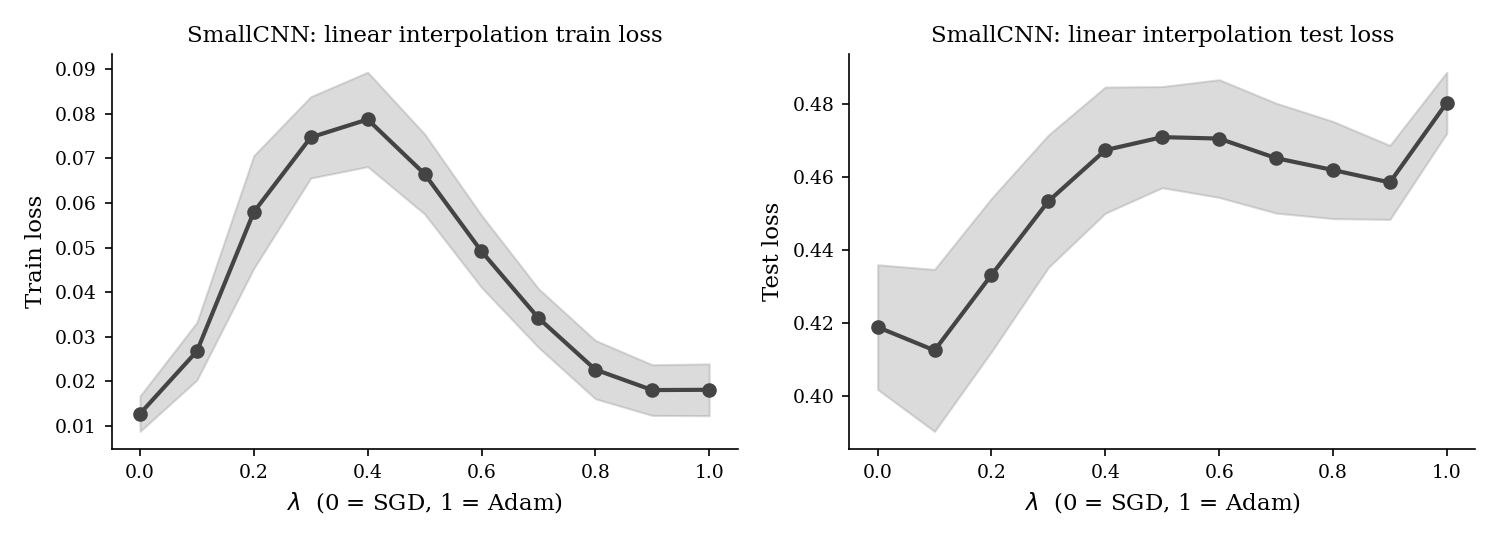
\includegraphics[width=\linewidth]{figures_extended/mode_connectivity_cnn.png}\caption{SmallCNN}\end{subfigure}
\caption{Linear mode connectivity: training and test loss along $\theta(\lambda)=(1-\lambda)\theta_{\mathrm{SGD}}+\lambda\theta_{\mathrm{Adam}}$, with BatchNorm recalibrated at interior $\lambda$. Solid line is mean over five matched seeds; band is $\pm 1$ std.}
\label{fig:mode-connectivity}
\end{figure}

\begin{table}[H]
\centering
\small
\begin{tabular}{lcc}
\toprule
\textbf{Model} & \textbf{Train barrier $B_{\text{train}}$} & \textbf{Test barrier $B_{\text{test}}$} \\
\midrule
MLP      & $0.0721 \pm 0.0086$ & $0.0174 \pm 0.0086$ \\
SmallCNN & $0.0615 \pm 0.0078$ & $0.0032 \pm 0.0065$ \\
\bottomrule
\end{tabular}
\caption{Loss barrier between matched SGD and Adam solutions along the linear interpolation. Mean $\pm$ std over five seeds.}
\label{tab:mode-connectivity}
\end{table}

The training-loss barriers are both small but consistently positive ($0.0721$ for the MLP, $0.0615$ for the SmallCNN), and substantially larger than the cross-seed standard deviations: there is a real, reproducible bump in training loss along the straight line connecting matched SGD and Adam solutions, even after BatchNorm recalibration. This is consistent with the two optimizers having selected distinct local minima rather than two points in the same flat basin, and it is consistent with the large parameter-space distances reported in Part~II being driven by basin-level rather than within-basin separation. The test-loss barriers are an order of magnitude smaller ($0.0174$ on the MLP and $0.0032$ on the SmallCNN, the latter statistically indistinguishable from zero), which says that the two basins, although separated on the training surface, agree closely on the test distribution. The basin separation we detect is therefore a feature of the empirical risk landscape, not of the population-risk landscape.

\FloatBarrier

% =============================================================================

\section{Part VIII: Function-Space Similarity}
\label{sec:function-space}

\subsection{Motivation}

Parameter-space distance does not directly measure how different the trained networks are as functions. Two networks can have very different parameter vectors and still produce nearly identical predictions on the data distribution, especially in the presence of scale symmetries and BatchNorm. To check whether the optimizer-induced parameter differences carry through to functional differences, we evaluate three function-level metrics on the test set.

\subsection{Metrics}

For matched SGD and Adam models with predicted class probabilities $p_S(\cdot|x)$ and $p_A(\cdot|x)$ and pre-softmax logits $z_S(x), z_A(x)$, we compute, over the $N$-point test set:
\begin{align}
D_{\mathrm{pred}} &= \frac{1}{N}\sum_{i=1}^N \mathbf{1}\!\big[\arg\max_k p_S(k|x_i)\ne \arg\max_k p_A(k|x_i)\big],\\
D_{\mathrm{SKL}} &= \frac{1}{2N}\sum_{i=1}^N \big[D_{\mathrm{KL}}(p_S\|p_A) + D_{\mathrm{KL}}(p_A\|p_S)\big],\\
C_{\mathrm{logit}} &= \frac{1}{N}\sum_{i=1}^N \frac{z_S(x_i)^\top z_A(x_i)}{\|z_S(x_i)\|_2\,\|z_A(x_i)\|_2}.
\end{align}
$D_{\mathrm{pred}}$ is a strict decision-level disagreement; $D_{\mathrm{SKL}}$ measures the divergence of the full softmax distribution; $C_{\mathrm{logit}}$ is scale-invariant and captures direction similarity in logit space.

\subsection{Results}

Table~\ref{tab:function-space} reports the three metrics.

\begin{table}[H]
\centering
\small
\begin{tabular}{lccc}
\toprule
\textbf{Model} & $D_{\mathrm{pred}}$ & $D_{\mathrm{SKL}}$ & $C_{\mathrm{logit}}$ \\
\midrule
MLP      & $0.0738 \pm 0.0028$ & $0.1749 \pm 0.0051$ & $0.6122 \pm 0.0058$ \\
SmallCNN & $0.0671 \pm 0.0042$ & $0.2676 \pm 0.0219$ & $0.6516 \pm 0.0061$ \\
\bottomrule
\end{tabular}
\caption{Function-space similarity between matched SGD and Adam models on the Fashion-MNIST test set. Mean $\pm$ std over five seeds.}
\label{tab:function-space}
\end{table}

The two optimizers disagree on $7.4\%$ of MLP test predictions and $6.7\%$ of SmallCNN predictions, considerably more than the residual seed-to-seed disagreement that would arise from numerical noise alone. Logit-direction cosine similarity is $\sim 0.61$--$0.65$ for both architectures, far below the value $\approx 1.0$ one would obtain comparing a model to itself; the trained predictors are correlated but distinguishably different. The architecture comparison adds structure: the SmallCNN has slightly lower $D_{\mathrm{pred}}$ but \emph{higher} $D_{\mathrm{SKL}}$ than the MLP, which means the CNN's two predictors agree more often on the argmax label but, when they differ in their full softmax distribution, do so more confidently. Function-level disagreement is therefore not absorbed by the convolutional inductive bias---it persists with comparable magnitude across both architectures, and the factor-three parameter distance from Part~II propagates into a measurable functional gap rather than being washed out by parameter symmetries.

\FloatBarrier
\begin{figure}[H]
\centering
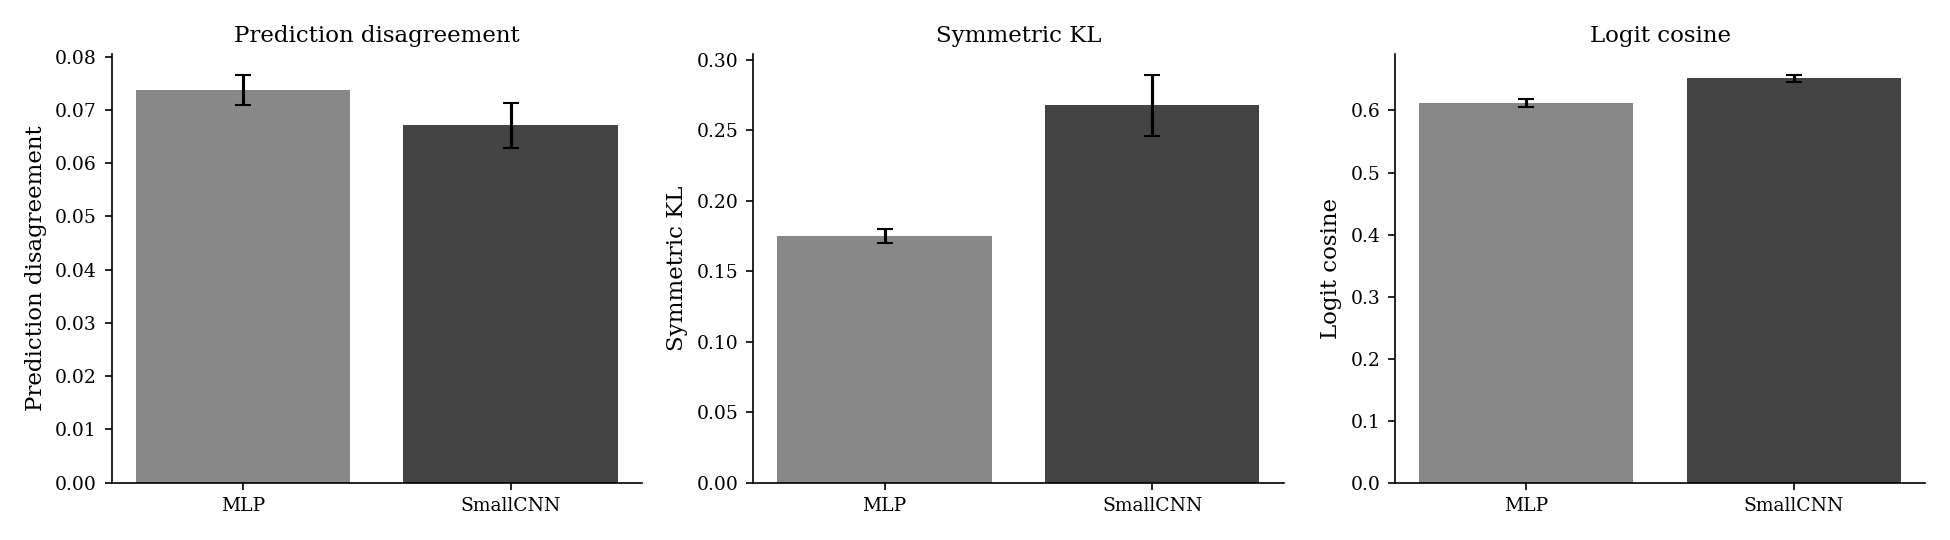
\includegraphics[width=0.6\linewidth]{figures_extended/function_space_bars.png}
\caption{Function-space disagreement metrics on Fashion-MNIST test set, mean $\pm$ std over five seeds.}
\label{fig:function-space-bars}
\end{figure}

\FloatBarrier

% =============================================================================

\section{Part IX: Representation-Space Geometry}
\label{sec:representation-space}

\subsection{Motivation}

Function-space metrics treat the network as a black box that maps inputs to outputs. Two networks with similar outputs may still rely on quite different internal feature representations. To probe this, we extract penultimate-layer features and compare their geometry.

For each architecture we fix the penultimate-layer module: in the MLP, the ReLU after the last hidden Linear; in the SmallCNN, the ReLU after the last hidden Linear in the classifier. For a test subset $\{x_i\}_{i=1}^n$ with $n=1024$, denote the feature matrix $F\in\mathbb{R}^{n\times d}$ where $d=128$ for both architectures.

\subsection{Two Alignment Measures}

\paragraph{Feature kernel alignment.} Form the cosine-normalized Gram matrix $K_\theta(i,j) = h_\theta(x_i)^\top h_\theta(x_j) / (\|h_\theta(x_i)\|\|h_\theta(x_j)\|)$ and compute
\[
A(K_S,K_A) = \frac{\langle K_S, K_A\rangle_F}{\|K_S\|_F\,\|K_A\|_F}.
\]
$A=1$ when the two Grams are scalar multiples of each other.

\paragraph{Linear CKA.} Linear centered kernel alignment \cite{kornblith2019similarity} is invariant to invertible linear transforms of the features and to isotropic scaling:
\[
\mathrm{CKA}(F_S,F_A) = \frac{\|\tilde F_S^\top \tilde F_A\|_F^2}{\|\tilde F_S^\top \tilde F_S\|_F\,\|\tilde F_A^\top \tilde F_A\|_F},
\]
where $\tilde F$ is column-centered.

\subsection{Results}

Table~\ref{tab:representation} reports $A$ and CKA between matched SGD and Adam features.

\begin{table}[H]
\centering
\small
\begin{tabular}{lcc}
\toprule
\textbf{Model} & \textbf{Feature kernel alignment $A$} & \textbf{Linear CKA} \\
\midrule
MLP      & $0.9697 \pm 0.0010$ & $0.8578 \pm 0.0059$ \\
SmallCNN & $0.9664 \pm 0.0027$ & $0.9147 \pm 0.0113$ \\
\bottomrule
\end{tabular}
\caption{Representation-space alignment between matched SGD and Adam penultimate-layer features on $n=1024$ test samples. Mean $\pm$ std over five seeds.}
\label{tab:representation}
\end{table}

Both alignment measures are high in absolute terms. Feature-kernel alignment is $\approx 0.97$ in both architectures, and linear CKA is $0.858$ for the MLP and $0.915$ for the SmallCNN. Despite Adam's parameters being $\sim 3\times$ farther from initialization than SGD's (Section~\ref{sec:path-length}) and the two solutions sitting in distinguishable training-loss basins (Section~\ref{sec:mode-connectivity}), the penultimate-layer feature geometries they induce are highly similar. The SmallCNN shows higher CKA than the MLP, in line with the expectation that the convolutional inductive bias compresses optimizer-induced effects toward the parameter level and away from the representation level: the convolutional structure forces both optimizers into nearly the same feature space, while the MLP allows the choice of optimizer to express itself more in the representation. The combination of high CKA ($\sim 0.86$--$0.91$) with non-trivial decision-level disagreement ($D_{\mathrm{pred}} \sim 0.07$ from Section~\ref{sec:function-space}) means similar features feed into measurably different decision boundaries: the optimizer-induced functional spread is concentrated in the final classifier rather than in the upstream representation.

\begin{figure}[H]
\centering
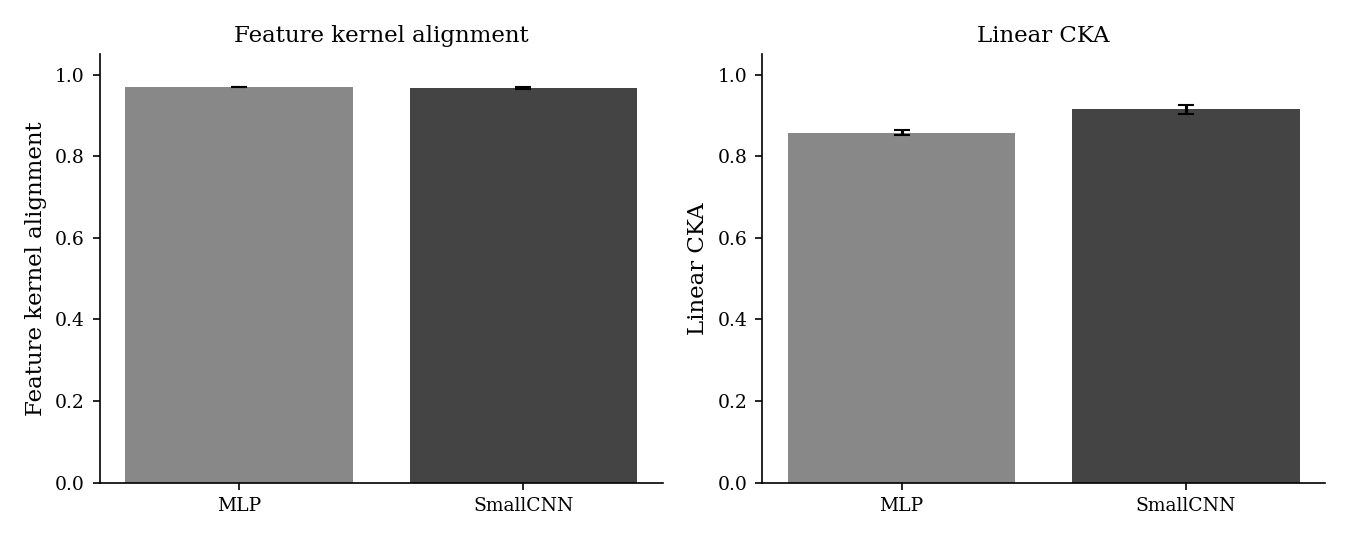
\includegraphics[width=0.55\linewidth]{figures_extended/representation_cka_bars.png}
\caption{Penultimate-layer feature similarity between matched SGD and Adam runs.}
\label{fig:representation-bars}
\end{figure}

\FloatBarrier

% =============================================================================

\section{Three-Level Synthesis}
\label{sec:three-level}

The Parts~II--IX sequence organizes evidence at three levels of geometry. Table~\ref{tab:three-level} summarizes the picture.

\begin{table}[H]
\centering
\small
\setlength{\tabcolsep}{3pt}
\begin{tabular}{p{2.4cm}p{4.8cm}p{4.5cm}p{3.5cm}}
\toprule
\textbf{Level} & \textbf{Quantities} & \textbf{What it answers} & \textbf{Verdict (this study)} \\
\midrule
Parameter geometry & $\|\theta_T-\theta_0\|_2$, $\mathcal{P}_T$, $R_T$, $\lambda_{\max}(H)$, $\operatorname{tr}(H)$, $\bar d_{\mathrm{seed}}$, $\Delta\widehat L(\sigma)$ & Where does the optimizer go, and what is the local curvature? & Adam path length $\sim 3\times$ SGD's in both architectures; directness ratio essentially equal. MLP: Adam $\sim 5$--$6\times$ flatter at matched loss. SmallCNN: ordering reverses---Adam $\sim 10\times$ \emph{sharper} at matched loss. \\
\addlinespace
Basin geometry & Linear-interpolation loss curve, barrier $B$ & Are the two solutions in the same low-loss region? & Small but reproducibly positive train barrier ($0.072$ MLP, $0.062$ CNN); test barrier $\le 0.02$. Distinct training-loss basins, near-identical population-loss landscape. \\
\addlinespace
Function and representation geometry & $D_{\mathrm{pred}}$, $D_{\mathrm{SKL}}$, $C_{\mathrm{logit}}$, $A(K_S,K_A)$, CKA & Do parameter differences correspond to different predictors or representations? & Decisions: $\sim 7\%$ disagreement and $C_{\mathrm{logit}}\approx 0.6$ in both. Representations: CKA $0.86$ MLP, $0.91$ CNN---high but not identical. Optimizer-induced functional spread is concentrated in the classifier head, not the feature space. \\
\bottomrule
\end{tabular}
\caption{Three-level synthesis of the implicit-bias evidence.}
\label{tab:three-level}
\end{table}

The data support a sharper version of the message we anticipated:
\begin{quote}
\emph{Adam substantially changes parameter-space trajectory and local Euclidean geometry, the change survives loss-matching control, and it crosses a (small) basin boundary on the training surface. But the change \textbf{compresses} as it propagates: by the function level, agreement is much closer ($\sim 93\%$); by the population-loss landscape, the two basins are essentially the same. The MLP/SmallCNN comparison shows that architecture also mediates which curvature regime each optimizer selects, with the convolutional inductive bias even reversing the flatness ordering at matched loss.}
\end{quote}

This is the core message of the extended report. Optimizer-induced parameter geometry is real and not merely a final-loss artifact; but generalization is determined by what survives at the function and representation levels, and by that point most of the parameter-space gap has been absorbed.

\FloatBarrier
\begin{figure}[H]
\centering
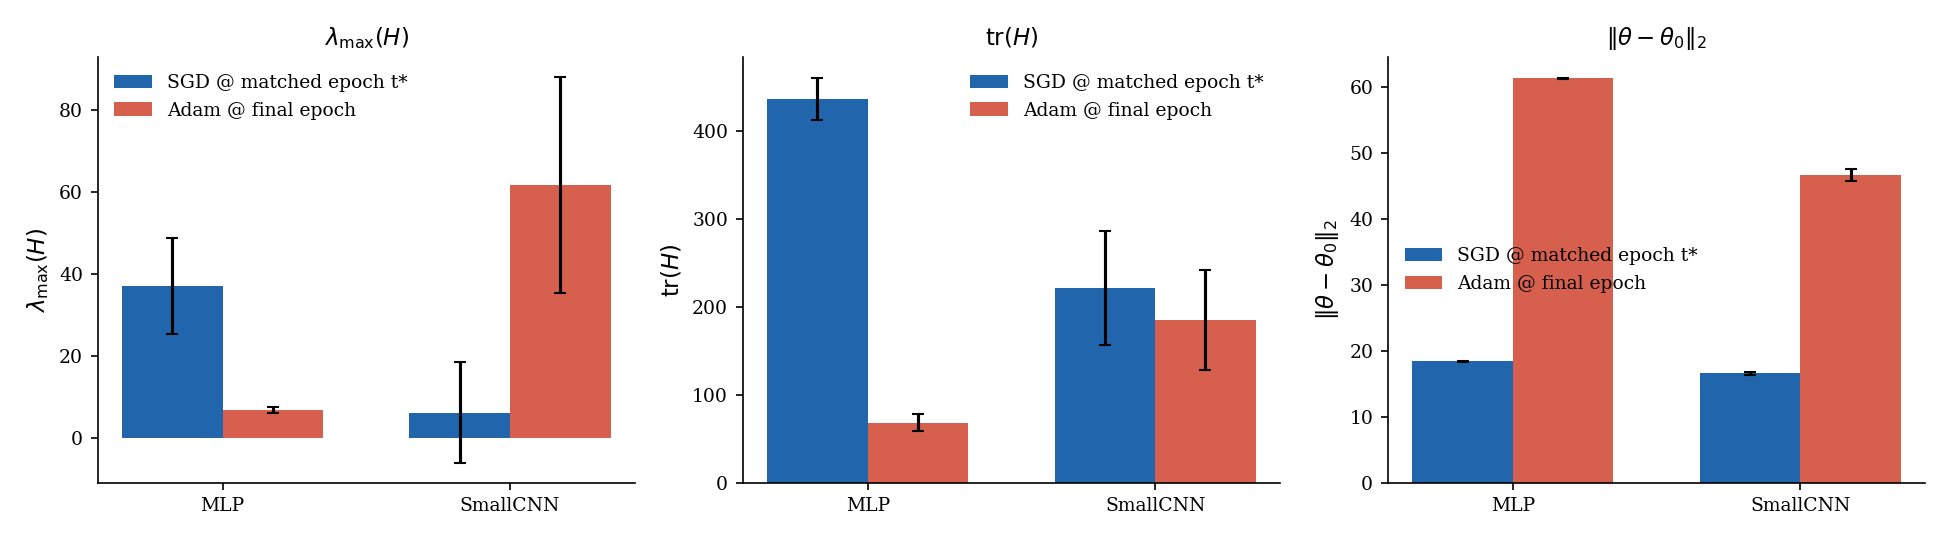
\includegraphics[width=0.85\linewidth]{figures_extended/loss_matched_summary.png}
\caption{Loss-matched geometry comparison across both architectures, summarizing $\|\theta-\theta_0\|_2$, $\lambda_{\max}(H)$, $\operatorname{tr}(H)$ and function-space disagreement.}
\label{fig:loss-matched-summary}
\end{figure}

\FloatBarrier


\section{Overall Discussion}

\subsection{Answer to the Main Question}

The main question was whether adaptive optimizers alter the implicit bias and generalization of neural networks. Based on these experiments, the answer is:
\begin{quote}
\emph{Yes, adaptive optimization alters the training trajectory and selected solution geometry, but this does not automatically imply better or worse generalization.}
\end{quote}

The clearest evidence for altered implicit bias is geometric. Adam moves much farther from initialization in both architectures and produces more dispersed final parameter vectors across seeds. These differences appear even when both optimizers fit the training set well. This supports the view that Adam is not just SGD with a faster clock, and that the two optimizers select different parameter-space regions of the loss landscape.

The MLP result is the clearest example. There, Adam is faster and is associated with solutions that are $5\times$ flatter by $\lambda_{\max}$ and $6\times$ lower in $\operatorname{tr}(H)$. Yet SGD achieves marginally higher test accuracy ($89.01\%$ vs.\ $88.87\%$) and a marginally smaller train--test gap ($9.04\%$ vs.\ $9.12\%$). Because these generalization differences are small relative to seed-to-seed variation, we do not interpret them as a strong optimizer ranking. The safer conclusion is that Adam's different trajectory and flatter MLP geometry do not translate into a clear test-accuracy or gap advantage.

The CNN weakens the simple version of this story further. Adam still moves farther from initialization and remains more dispersed across seeds, but final test accuracy and train--test gap stay within seed-to-seed variation. Curvature proxies are mixed rather than cleanly favoring Adam. This pattern is consistent with architecture mediating optimizer-induced differences. Convolutional structure, local receptive fields, and weight sharing may impose a stronger inductive bias than the choice between Adam and SGD in this Fashion-MNIST setting, but our experiments should not be read as a causal proof of that mechanism.

\subsection{Why the MLP and CNN Differ}

The MLP has fewer built-in structural assumptions about images. It treats the input as a vector, so the optimizer has more freedom to choose among many functionally different parameter configurations. In this setting, optimizer implicit bias is easier to observe. Adam's coordinate-wise normalization changes the trajectory, and this difference remains visible in curvature, even though it does not produce a reliable generalization advantage.

The CNN already encodes useful image priors through convolution and pooling. These architectural choices reduce the burden on the optimizer by restricting the function class toward translation-aware local feature extraction. As a result, both optimizers may find similarly good classifiers even if their parameter vectors differ substantially. This is consistent with Adam moving farther in parameter space without producing a meaningful test-accuracy advantage.

\subsection{Why Geometry Does Not Always Predict Generalization}

The MLP/CNN comparison shows that geometry is informative but not decisive on its own. A low sharpness value can indicate local robustness in parameter space, but test accuracy depends on the function learned by the network and on how well that function matches the data distribution. Architecture can strongly shape this function class. In the CNN, local filters and weight sharing already encode useful assumptions about images, so both optimizers can learn functions that generalize similarly even when their parameter vectors and curvature proxies differ.

Another reason geometry may fail to predict generalization perfectly is that the measured quantities are local and approximate. Sharpness and trace are computed at the endpoint, on a minibatch, and in the coordinates of the current parameterization. Generalization, by contrast, is a global property of the learned classifier on unseen data. A local curvature proxy need not correlate with generalization even within a single dataset. Our MLP results illustrate this point: the flatter optimizer (Adam) does not generalize better than the sharper optimizer (SGD). This is why our final claim is deliberately conditional: adaptive optimization changes the selected solution geometry, but the effect of that geometry on test performance depends on the surrounding modeling choices, and may run counter to naive flat-minima intuition.

\subsection{Relation to Existing Literature}

The results partially align with the literature on adaptive methods, but they also show that the practical story is nuanced. Wilson et al. \cite{wilson2017marginal} emphasize that adaptive methods may generalize worse than SGD in some problems. Our MLP results are directionally consistent with this concern: Adam finds substantially flatter solutions yet has marginally lower mean test accuracy and a slightly larger mean train--test gap than SGD, although these differences are small relative to seed variation. Our results also agree with the broader point that optimizer choice changes solution selection in geometrically meaningful ways.

The MLP results challenge a simple flat-minima interpretation \cite{hochreiter1997flat,keskar2017large} at the cluster level: the optimizer with lower Hessian sharpness (Adam) does not achieve a smaller train--test gap. The CNN results reinforce the caution raised by Dinh et al. \cite{dinh2017sharp}: sharpness is not a universal standalone predictor of generalization, and its relationship to test performance can be reversed or absent depending on the architecture and scale.

\subsection{Limitations}

Several limitations matter for interpreting the results.

\begin{enumerate}
    \item \textbf{Single dataset.} All experiments use Fashion-MNIST. The conclusions may differ on CIFAR, language modeling, or larger-scale vision tasks.
    \item \textbf{Limited architectures.} We compare only one MLP and one small CNN. More architectures would be needed to map how architectural inductive bias interacts with optimizer bias.
    \item \textbf{Five seeds.} Five seeds are enough to reveal stable large effects, such as Adam's parameter-distance difference, but they are not enough for fine-grained statistical claims.
    \item \textbf{Sharpness is a proxy.} We estimate Hessian sharpness and trace on a mini-batch. These quantities are computationally useful but not exact full-dataset curvature measures.
    \item \textbf{BatchNorm and scaling.} Both models use BatchNorm. Because neural networks can have scale symmetries, absolute sharpness values should be interpreted cautiously.
    \item \textbf{Hyperparameter dependence.} The learning-rate search shows that SGD can become much stronger when tuned. Therefore, the default comparison should not be read as a universal optimizer ranking.
    \item \textbf{No regularization or augmentation.} The main experiments use no weight decay, dropout, or data augmentation. These choices make optimizer effects easier to see, but they are not a full production training recipe.
\end{enumerate}

\subsection{What Would Strengthen the Study}

If we had more time, the most useful extensions would be running the label-noise and small-data experiments already specified in the configuration files, adding a broader learning-rate grid for both optimizers, comparing AdamW separately from Adam, and repeating the analysis on a more difficult dataset such as CIFAR-10. It would also be useful to compute additional geometry measures that are less sensitive to reparameterization, such as normalized sharpness or perturbation-based PAC-Bayes-style flatness metrics \cite{neyshabur2017exploring}.

\section{Conclusion}

This project compared SGD and Adam across three linked questions: convergence speed, implicit solution geometry, and generalization. The experiments show that Adam has a clear early-stage convergence advantage over the default SGD baseline, especially in the MLP. They also show that Adam and SGD converge to different parameter-space regions: Adam moves farther from initialization and produces more dispersed final solutions across seeds.

The generalization story is more nuanced. In the MLP, Adam finds substantially flatter solutions by Hessian-based proxies, yet SGD achieves marginally higher test accuracy ($89.01\%$ vs.\ $88.87\%$) and a marginally smaller train--test gap ($9.04\%$ vs.\ $9.12\%$). This shows that flatter geometry does not automatically give a generalization advantage. In the SmallCNN, optimizer-induced curvature differences are mixed, while generalization stays within seed-to-seed variation. The conclusion, then, is that in our tested setting, Adam appears to alter the implicit bias of training, but the effect on generalization is not determined by flatness alone; it is mediated by architecture, scale, and tuning. The most accurate conclusion is not "Adam is better" or "SGD generalizes better." Instead, optimizer adaptivity changes the path through the loss landscape. Whether that geometric difference matters for test performance depends on how much freedom the architecture leaves for the optimizer to choose among solutions.

\begin{thebibliography}{9}

\bibitem{kingma2015adam}
Diederik P. Kingma and Jimmy Ba.
\newblock Adam: A Method for Stochastic Optimization.
\newblock International Conference on Learning Representations, 2015.
\newblock \url{https://arxiv.org/abs/1412.6980}.

\bibitem{soudry2018implicit}
Daniel Soudry, Elad Hoffer, Mor Shpigel Nacson, Suriya Gunasekar, and Nathan Srebro.
\newblock The Implicit Bias of Gradient Descent on Separable Data.
\newblock Journal of Machine Learning Research, 19(70):1--57, 2018.
\newblock \url{https://jmlr.org/papers/v19/18-188.html}.

\bibitem{hochreiter1997flat}
Sepp Hochreiter and J\"urgen Schmidhuber.
\newblock Flat Minima.
\newblock Neural Computation, 9(1):1--42, 1997.
\newblock \url{https://doi.org/10.1162/neco.1997.9.1.1}.

\bibitem{keskar2017large}
Nitish Shirish Keskar, Dheevatsa Mudigere, Jorge Nocedal, Mikhail Smelyanskiy, and Ping Tak Peter Tang.
\newblock On Large-Batch Training for Deep Learning: Generalization Gap and Sharp Minima.
\newblock International Conference on Learning Representations, 2017.
\newblock \url{https://openreview.net/forum?id=H1oyRlYgg}.

\bibitem{dinh2017sharp}
Laurent Dinh, Razvan Pascanu, Samy Bengio, and Yoshua Bengio.
\newblock Sharp Minima Can Generalize For Deep Nets.
\newblock International Conference on Machine Learning, 2017.
\newblock \url{https://proceedings.mlr.press/v70/dinh17b.html}.

\bibitem{wilson2017marginal}
Ashia C. Wilson, Rebecca Roelofs, Mitchell Stern, Nati Srebro, and Benjamin Recht.
\newblock The Marginal Value of Adaptive Gradient Methods in Machine Learning.
\newblock Advances in Neural Information Processing Systems, 2017.
\newblock \url{https://proceedings.neurips.cc/paper/2017/hash/81b3833e2504647f9d794f7d7b9bf341-Abstract.html}.

\bibitem{neyshabur2017exploring}
Behnam Neyshabur, Srinadh Bhojanapalli, David McAllester, and Nati Srebro.
\newblock Exploring Generalization in Deep Learning.
\newblock Advances in Neural Information Processing Systems, 2017.
\newblock \url{https://proceedings.neurips.cc/paper_files/paper/2017/hash/10ce03a1ed01077e3e289f3e53c72813-Abstract.html}.

\bibitem{garipov2018loss}
Timur Garipov, Pavel Izmailov, Dmitrii Podoprikhin, Dmitry P. Vetrov, and Andrew Gordon Wilson.
\newblock Loss Surfaces, Mode Connectivity, and Fast Ensembling of DNNs.
\newblock Advances in Neural Information Processing Systems, 2018.
\newblock \url{https://proceedings.neurips.cc/paper/2018/hash/be3087e74e9100d4bc4c6268cdbe8456-Abstract.html}.

\bibitem{frankle2020linear}
Jonathan Frankle, Gintare Karolina Dziugaite, Daniel M. Roy, and Michael Carbin.
\newblock Linear Mode Connectivity and the Lottery Ticket Hypothesis.
\newblock International Conference on Machine Learning, 2020.
\newblock \url{https://proceedings.mlr.press/v119/frankle20a.html}.

\bibitem{kornblith2019similarity}
Simon Kornblith, Mohammad Norouzi, Honglak Lee, and Geoffrey Hinton.
\newblock Similarity of Neural Network Representations Revisited.
\newblock International Conference on Machine Learning, 2019.
\newblock \url{https://proceedings.mlr.press/v97/kornblith19a.html}.

\end{thebibliography}

\end{document}
